%!TEX root = ../template.tex
%%%%%%%%%%%%%%%%%%%%%%%%%%%%%%%%%%%%%%%%%%%%%%%%%%%%%%%%%%%%%%%%%%%%
%% chapter5_PrototypingPerf.tex
%% NOVA thesis document file
%%
%% Chapter with the Prototyping and Performance Evaluation Results part
%%%%%%%%%%%%%%%%%%%%%%%%%%%%%%%%%%%%%%%%%%%%%%%%%%%%%%%%%%%%%%%%%%%%

\typeout{NT FILE chapter5_PrototypingPerf.tex}

\chapter{Prototyping and Functional Evaluation Results}\label{cha:chapter5_PrototypingPerf}

%So neste capitulo e que se deve descrever a operacao do circuito.
Upon completion of the circuit design phase, the next step starts to dictate the physical shape of the prototype.

\section{PCB Layout}\label{sec:51_PCBlayout} % se calhar tiro "Design"
%provavelmente este capitulo deve ficar no final do Chapter 4, porque layout também é hardware design

\subsection{Footprint Assignment and Placement}\label{sec:511_Placement}

Once the all circuits' schematics that make up the system are correctly designed, every component symbol is referenced, and the KiCad's Electrical Rules Checker (ERC) has been ran, reporting no errors nor warnings (Figure~\ref{fig:ERC_errors}), the process of footprint assignment for the parts can start. KiCad provides a footprint assignment tool, to attribute the desired footprints to the project's parts.
\begin{figure}[h]
	\centering
	\includegraphics[width=0.6\textwidth]{Chapters/Figures/chapter5/ERC.png}
	\caption{KiCad's Electrical Rules Checker ran for all the finalized system's circuit schematics.}
	\label{fig:ERC_errors}
\end{figure}
Since the new beRTK\textsuperscript{\textregistered} circuit is based around fourteen main ICs and modules, selecting the correct footprints for each of these was the starting point for the layout phase. For that, datasheets for ICs and modules usually feature a section dedicated to presenting the recommended footprint for their component. This facilitates designers' work, as KiCad already provides a vast list of footprint libraries with many footprints to choose from, and therefore the attribution boiled down to a simple matter of finding the correct matches, referring to the datasheets. Figure~\ref{fig:footprint_AP64501} shows the recommended solder pad pitch and dimensions for the AP64501 buck converter addressed in Section~\ref{sec:3214_AP64501}, an example of what is taken as reference when assigning footprints.

% meter aqui footprint LTC4012 - datasheet
\begin{figure}[h]
	\centering
	\includegraphics[width=0.7\textwidth]{Chapters/Figures/chapter5/footprint_AP64501.pdf}
	\caption{Recommended solder pad pitch and dimensions for the AP64501 synchronous buck converter~\cite{AP64501}.}
	\label{fig:footprint_AP64501}
\end{figure}

For the ICs and modules whose footprints are not provided by default by the software, internet research was conducted in order to find them -- \url{https://www.snapeda.com/} and \url{https://pt.mouser.com/} were the two websites accessed for such purpose, since these are known to provide trustworthy footprints.

As a design rule for this project, regarding resistors, unless otherwise stated, all should have a 0805 \gls{SMD} package footprint and a tolerance of 5\%. The standard 0805 package size measures $0.08 \times 0.05$ inches (length $\times$ width), which corresponds, in the metric system, to a 2012 package size, at $2.0 \times 1.25$ millimetres (length $\times$ width).
Capacitors should also have a 0805 SMD package footprint and be rated for 50V, unless otherwise stated. It should be noted that, for these package's footprints, a version labelled ``HandSolder'' (in KiCad) was selected. This was done in order to aid the hand soldering parts of the prototype assembly phase, since for these the footprint, the package's pads are made slightly wider.

As for the remaining components, i.e. MOSFETs, diodes, inductors, ferrites, crystal and connectors, their footprint depends on the application.
Datasheets of ICs and modules usually refer the characteristics and/or models to use in a typical implementation.

To effectively design the board's layout, KiCad provides a PCB editor that places the assigned footprints in single editing window. This premature placement must then be rearranged according to the respective component's location in the circuit, in the most efficient way possible among other partner components. The PCB editor also displays white lines (known as ``ratsnest lines'') that connect the different components' pads to each other, just as defined in the schematic design. This subsequently helps in the routing process (i.e. effectively connecting every component with tracks (also known as ``traces''), vias and zones). Figure~\ref{fig:ratsnest} shows an early version of the layout for the external power supply region of the system, which is connected to the LTC4012 and to the external power voltage reference (top left area of the schematic of Figure~\ref{fig:LTC4012_circuit}).

\begin{figure}[h]
	\centering
	\includegraphics[width=0.8\textwidth]{Chapters/Figures/chapter5/ratsnest.png}
	\caption{Unconnected footprints for the external power supply region of the system (early version).}
	\label{fig:ratsnest}
\end{figure}


%s--Ss--Ss--Ss--Ss--Ss--Ss--Ss--Ss--Ss--Ss--Ss--Ss--Ss--Ss--Ss--Ss--Ss--Ss--S
\subsubsection{Control Unit and USB 2.0 Hub}\label{sec:5111_CM4_LAN9514}

%0. falar do placement estar concluido:
To arrange all components in the best way possible, one has to take into account a provisional routing, to achieve a good placement in the least amount of iterations possible. For that, it's considered good practice to start by imagining and experimenting with placing and routing of the high-speed zones of the circuit first. For this project, that would concern the CM4's high-speed side and the LAN9514's USB side. Figure~\ref{fig:placement_CM4_LAN9514} focuses on the final component placement of the CM4 module and the LAN9514 hub on the board.

\begin{figure}[h]
	\centering
	\includegraphics[width=0.7\textwidth]{Chapters/Figures/chapter5/placement_CM4_LAN9514.png}
	\caption{Final placement of the CM4 and LAN9514 circuits' components.}
	\label{fig:placement_CM4_LAN9514}
\end{figure}%placement_CM4_LAN9514

The location of the peripheral ports (HDMI and USB) must also be accounted for. It is common for these to be placed near the limits of the board so that user access is facilitated.

After placing the downstream USB connectors near the right edge of the board, the LAN9514 hub was placed to the left of these, in way that it would be more-or-less equidistant from each to account for the routing of the high-speed USB data traces. After defining a position for the hub, its most important component was placed: the crystal oscillator XT1. This part must be the closest possible to its respective hub's pins, in order to settle a trustworthy clock frequency from which the IC will rely on. Followed by the crystal's capacitors, the remaining components were placed the nearest possible to the hub.

Setting the CM4 immediately to the left of the USB hub, choosing to locate the HDMI port on the left edge of the board, near the CM4's HDMI pins, was straightforward.

The power and activity LEDs (D15 and D14, respectively) were placed near the top left edge of the board (i.e. top left of Figure~\ref{fig:placement_CM4_LAN9514}), a simple and easy-to-remind location, specially for the testing phase.

All the CM4's test points (e.g. +3V3, WL\_nDisable, GPIOx, etc.) are located either near the top or bottom of the module (MOD1) -- also easy-to-remind and to reach locations.

Regarding the LAN9514's bypass capacitors, these were placed near the top-middle of the board, as well as above and below the downstream USB connectors (also visible in Figure~\ref{fig:placement_CM4_LAN9514}).


%s--Ss--Ss--Ss--Ss--Ss--Ss--Ss--Ss--Ss--Ss--Ss--Ss--Ss--Ss--Ss--Ss--Ss--Ss--S
\subsubsection{Power Selector and Battery Balancer}\label{sec:5112_LTC4012_BQ29209}

The next step taken was the placement of the power selector circuit. In the applications information sections of the LTC4012 datahseet (\cite{LTC4012}), a list of PCB layout considerations are provided. Regarding these, it is recommended to follow a specific priority order, as to ensure a proper layout. The notes go through the best possible layout for the switch node of the battery charger and its importance in the design. This switch node corresponds to the point where diode D4 and inductor L1 meet (see Figure~\ref{fig:LTC4012_circuit}), and is directly connected to pin SW of the LTC4012. The suggested priority list for the LTC4012 layout starts with notes on the correct placement of the switching FETs (Q2 and Q9) relative to the IC and its input capacitors, running through the inductor, current sense resistors, output capacitors and notes regarding PCB layer, trace and via topology. Following these guidelines resulted in the component placement represented on the right side of Figure~\ref{fig:placement_Power_Selector_and_BQ29209}, where the switching FETs, input capacitors and inductor are clearly visible close and around the LTC4012 footprint.

%placement_Power_Selector_and_BQ29209
\begin{figure}[h]
	\centering
	\includegraphics[width=0.7\textwidth]{Chapters/Figures/chapter5/placement_Power_Selector_and_BQ29209.png}
	\caption{Final placement of the Power Selector and Battery Balancer circuits' components.}
	\label{fig:placement_Power_Selector_and_BQ29209}
\end{figure}

BQ29209's datasheet (\cite{bq29209}) also provides a dedicated section highlighting recommended layout suggestions for users. Among other notes, these encourage the designer to place the input capacitors as close as possible to the IC in order to filter out the most amount of noise possible. This resulted in the placement shown on the lower left-hand side of Figure~\ref{fig:placement_Power_Selector_and_BQ29209}.


%s--Ss--Ss--Ss--Ss--Ss--Ss--Ss--Ss--Ss--Ss--Ss--Ss--Ss--Ss--Ss--Ss--Ss--Ss--S
\subsubsection{Voltage Converter}\label{sec:5114_VoltageConverter}

Similar to the previous IC's datasheets,~\cite{AP64501} singles important guidelines for a thorough layout of the AP64501's circuit. These guidelines are laid out in list form, starting by addressing the recommended copper thickness for the carrier board for the IC (due to the maximum 5A output current), followed by the importance of the placement of the input capacitors and inductor (L2) as close as possible to their respective terminals on the converter. More specifically, the input capacitors should be placed close to the power supply (VIN) of the IC, and the inductor close to the switching terminal (SW) -- similar to the layout topology addressed by the LAN9514's datasheet. After this, the list focuses on output capacitors, feedback components, and finally PCB layers and vias. A layout schematic example is also provided, and is represented in Figure~\ref{fig:AP64501_layout_Datasheet}.

% meter aqui AP64501 layout - datasheet
\begin{figure}[h]
	\centering
	\includegraphics[width=0.5\textwidth]{Chapters/Figures/chapter5/AP64501_layout_Datasheet.pdf}
	\caption{Recommended layout for the AP64501 synchronous buck converter's circuit~\cite{AP64501}.}
	\label{fig:AP64501_layout_Datasheet}
\end{figure}

Taking all these notes into account resulted in the component placement depicted on Figure~\ref{fig:placement_VoltageConverter}.

%placement_VoltageConverter
\begin{figure}[h]
	\centering
	\includegraphics[width=0.6\textwidth]{Chapters/Figures/chapter5/placement_VoltageConverter.png}
	\caption{Final placement of the Voltage Converter circuit's components.}
	\label{fig:placement_VoltageConverter}
\end{figure}


%s--Ss--Ss--Ss--Ss--Ss--Ss--Ss--Ss--Ss--Ss--Ss--Ss--Ss--Ss--Ss--Ss--Ss--Ss--S
\subsubsection{Power Switch}\label{sec:5115_PowerSwitch}

The power switch circuit placement revealed itself to be very simple.
\cite{SN74LVC2G74DCTR} highlights that the unused inputs for the D-type flip-flop must be tied either to GND or VCC. Figure~\ref{fig:placement_PowerSwitch} shows the arrangement made for this circuit, which essentially surrounds the main ICs (the D-type flip-flop, the inverter, and the voltage regulator) with their function-defining components.

%placement_PowerSwitch
\begin{figure}[h]
	\centering
	\includegraphics[width=0.4\textwidth]{Chapters/Figures/chapter5/placement_PowerSwitch.png}
	\caption{Final placement of the Power Switch circuit's components.}
	\label{fig:placement_PowerSwitch}
\end{figure}


%s--Ss--Ss--Ss--Ss--Ss--Ss--Ss--Ss--Ss--Ss--Ss--Ss--Ss--Ss--Ss--Ss--Ss--Ss--S
\subsubsection{Human-Machine Interface}\label{sec:5116_HMI}

Figure~\ref{fig:placement_HMI} shows the placement of the LM2901 comparator's circuit (see left-hand side of Figure~\ref{fig:HMI_circuit}).
Placement for this part of the system also proved to be straightforward, due to the reduced number of components (mainly resistors), which were simply laid out around comparator U6.

As explained previously, the status voltage from the comparator flows to the HMI itself through the connection of two 2.54mm pitch pin headers, F4 and F5. F4 is placed close to U6, as well as to the top right corner of the board, on its opposite side (see Figure~\ref{fig:placement_HMI}, left). It is supposed to be connected to F5 to power all status-indication LEDs and push-button SW1, as well as to establish nets PWR\_SWITCH, PWR\_LED and EXT\_PWR. The right side of Figure~\ref{fig:placement_HMI} shows a small separate PCB just for the HMI. The reason for this separate board is due to its specific user-accessible location on the outside of the base station's casing.

%placement_HMI
\begin{figure}[h]
	\centering
	\includegraphics[width=0.8\textwidth]{Chapters/Figures/chapter5/placement_HMI.png}
	\caption{Final placement of the status voltage comparator (left) and HMI (right) circuits' components.}
	\label{fig:placement_HMI}
\end{figure}


%s--Ss--Ss--Ss--Ss--Ss--Ss--Ss--Ss--Ss--Ss--Ss--Ss--Ss--Ss--Ss--Ss--Ss--Ss--S
\subsubsection{GNSS module and Wi-Fi Transceiver}\label{sec:5117_ZED_XBEE}

Aside from connector F4, the GNSS module was the only system part to be placed on the back side of the main board, since this was the most convenient location due to its mechanical structure (i.e. because the module itself consists on a small PCB with a pin header soldered on it). The remaining components connected to the GNSS module's circuit, namely the RTK ISP connector, input capacitors C9 and C10, and diodes D6 and D7 are placed on the front side of the main board, near the opposite location of the module itself, along with the RTK data test points. All this can be seen on the top portion of the left side of Figure~\ref{fig:placement_ZED_XBEE}.

%placement_ZED_XBEE
\begin{figure}[h]
	\centering
	\includegraphics[width=0.8\textwidth]{Chapters/Figures/chapter5/placement_ZED_XBEE.png}
	\caption{Final placement of the GNSS module and Wi-Fi Transceiver circuits' components (left); Antenna keepout area for the XBee 3 RF module (right).}
	\label{fig:placement_ZED_XBEE}
\end{figure}

As for the Wi-Fi transceiver, i.e. the XBee 3 RF module,~\cite{XBee} provides layout design notes to help achieve the best antenna performance possible. Since the XBee module used in this project is known as the its ``micro chip'' version, the notes for this version are the ones to pay attention to. These state that non-metal enclosures are preferred, and that all metal parts of the system -- either internal or external in respect to the main board -- must be kept at the maximum distance possible from the module's antenna. For that,~\cite{XBee} also provides a graphic visualization of a recommended antenna keepout area to implement. In this area, only a copper pour and minimal routing (to connect the needed module's pins on that zone) are permitted. The right side of Figure~\ref{fig:placement_ZED_XBEE} shows such area (represented by a large rectangle).

After assessing these guidelines, the placement of this circuit's components was standard when compared to the previous sections, with output capacitors C11-C14 of the LDO U2 placed as close as possible to its output, as well as to the VCC input (pin 2) of the XBee module. All test points for the latter (DIO0-DIO3) are placed above it.

%   dizer que é importante o cristal estar mais perto possivel do LAN, porque o routing desta parte do circuito é critica;
%   importante as USB downstream ports estarem o mais perto possivel do LAN
%   ver se me lembro de mais regras...
%   definiu-se um limite experimental para a placa ($100 \times 70$ mm (length $\times$ width)) e acabou por se aumentar para $129 \times 90$ mm (length $\times$ width).

After the placement of every circuit, three fiducial markers were added on every corner of the main board but the top-right one. These markers serve as reference points for the PCB manufacturing machines.
With such, the remaining placement-related task was to assign these to roughly specific locations on the board. Choosing the board's dimensions settles the placement phase. For the main board, the final size was set to $129 \times 90$ mm (length $\times$ width). As for the HMI board, the same $30 \times 60$ mm (length $\times$ width) measurements from the previous beRTK\textsuperscript{\textregistered} version were kept unaltered. Figure~\ref{fig:placement_FULL} shows the final placement of the entire system within the board's defined limits.

%placement_FULL
\begin{figure}[h]
	\centering
	\includegraphics[width=0.6\textwidth]{Chapters/Figures/chapter5/placement_FULL.png}
	\caption{Final placement of the new beRTK\textsuperscript{\textregistered} system's circuit, within the board's defined limits.}
	\label{fig:placement_FULL}
\end{figure}


%sSsSsSsSsSsSsSsSsSsSsSsSsSsSsSsSsSsSsSsSsSsSsSsSsSsSsSsSsSsSsSsSsSsS
\subsection{Routing}\label{sec:52_Routing}

%   depois começa o routing:
After placement, routing is the process that connects every component to each other, and at the PCB level, this can either occur with traces, vias or copper pours.

\subsubsection{Board Setup}\label{sec:521_Board_Setup}

%1. falar das minimum design rules da eurocircuits:
Before beginning the routing process, the board setup must be done in the KiCad PCB editor. This critical step consists in defining the board's stack-up (i.e. number of copper layers -- or simply ``layers'' --, copper pour thickness) and design rules. Depending on the chosen PCB manufacturer, these definitions may vary. For this project, the selected board manufacturer was Eurocircuits, a ``specialist manufacturer and assembler of prototype and small series PCBs''\footnote[19]{Available at \url{https://www.eurocircuits.com/who-are-we/}.}. For KiCad users, Eurocircuits provides sets of minimum design rules (i.e. design constraints) for various PCB stack-up types that may vary in either single or double-sided designs, number of layers, or copper thickness. The following set of constraints presented are for a four-layer board with a base copper thickness of $18 \mu$m and $35 \mu$m, for the outer (OL) and inner (IL) layers, respectively\footnote[20]{Eurocircuits KiCad design rules for other board stack-ups are available at \url{https://www.eurocircuits.com/blog/kicad-design-rules/}.}:
\begin{itemize}
	\item Min. trace width, OL: 0.150mm;
	
	\item Min. clearance, OL: 0.150mm;
	
	\item Min. trace width, IL: 0.150mm;
	
	\item Min. clearance, IL: 0.150mm;

	\item Min. via drill diameter (tool size): 0.35mm;
	
	\item Min. via pad diameter, OL: 0.600mm;
	
	\item Min. via pad diameter, IL: 0.600mm.
\end{itemize}
Therefore, the board's stack-up defined by these constraints was selected as the stack-up for the new beRTK\textsuperscript{\textregistered}'s board. The four-layer order chosen (from front to back) was signal-power-power-signal (in this case: F.Cu-GND-PWR-B.Cu; F.Cu and B.Cu refer to the board's front and back copper signal layers).

A second Eurocircuits' tool can be used to obtain the board's physical stack-up dimensions -- the ``Buildup Editor''. This tool allows the user to select the board's desired number of layers, along with its thickness and base material (among other specifications), and provides a preview of its layers' stack-up with the expected physical dimensions in millimetres. Figure~\ref{fig:buildup_4layer} shows the Eurocircuits Buildup Editor's calculation of the physical stack-up for a four-layer, 1.55mm thick PCB with an FR-4 base material.

\begin{figure}[h]
	\centering
	\includegraphics[width=0.8\textwidth]{Chapters/Figures/chapter5/buildup_4layer.png}
	\caption{Eurocircuits Buildup Editor's calculation of the physical stack-up of a four-layer, 1.55mm thick PCB with an FR-4 Improved base material (available in the Eurocircuits website).}
	\label{fig:buildup_4layer}
\end{figure}

\noindent The values displayed in the diagram of Figure~\ref{fig:buildup_4layer} can thus be applied to the physical stack-up tab of KiCad's board setup manager, as shown in Figure~\ref{fig:KiCad_buildup_4layer}.

\begin{figure}[h]
	\centering
	\includegraphics[width=0.8\textwidth]{Chapters/Figures/chapter5/KiCad_buildup_4layer.png}
	\caption{Board's physical stack-up dimensions applied in KiCad's board setup manager.}
	\label{fig:KiCad_buildup_4layer}
\end{figure}

After setting up the physical stack-up of the board and defining its design rules' constraints, the net classes must be defined. For specified nets (e.g. VBAT, PWR\_LED, GPS\_VDD, etc.), these dictate the actual PCB trace's width and clearance, as well as the size of vias to use. To define a net's trace dimensions, key parameters such as its current flow capacity (in A) temperature rise above ambient ($\Delta T$, in $\degree$C), and copper resistivity ($1.72 \cdot 10^{-8} \Omega$m) must be taken into account. KiCad also provides a PCB calculator tool for trace width calculation, shown in Figure~\ref{fig:PCB_calculator}.

\begin{figure}[h]
	\centering
	\includegraphics[width=0.8\textwidth]{Chapters/Figures/chapter5/PCB_calculator.png}
	\caption{KiCad's PCB track width calculator used.}
	\label{fig:PCB_calculator}
\end{figure}

Looking at Figure~\ref{fig:PCB_calculator}, it is possible to see that the calculator accepts either parameter or layer trace dimension inputs. As stated in the figure, the IPC 2221 (the Generic Standard on Printed Board Design) formula to calculate the trace's maximum current allowed is given by (\ref{eq:I_trace}):

\begin{equation}\label{eq:I_trace}
	I = K \cdot \Delta T^{0.44} \cdot (W \cdot H)^{0.725}\,\medskip
\end{equation}
\noindent Where:
\begin{itemize}
	\item $I$ -- Maximum current that will flow through the trace, in A;
	
	\item $\Delta T$ -- Temperature rise above ambient, in $\degree$C;
	
	\item $W$ -- Trace width, in mils (1 mils $=$ 0.0254 millimeters);
	
	\item $H$ -- Trace thickness (i.e. height), in mils;
	
	\item $K$ -- 0.024 for internal traces or 0.048 for external traces.
\end{itemize}

For this project, four net classes were defined for the routing process:

\begin{itemize}
	\item Default net class -- Corresponds to every net in the circuit that is not HDMI, USB, or power-related. Examples for such are the nets that connect each of the four outputs of comparator U6 to pin header F4, for the status voltage (Figure~\ref{fig:HMI_circuit});
	
	\item Power net class -- Corresponds to every net in the circuit where considerable amount of current is expected to flow. Examples for such are the PWR\_LTC and 5V nets;
	
	\item USB net class -- Corresponds to every USB-related net in the circuit;
	
	\item HDMI net class -- Corresponds to every HDMI-related net in the circuit.
\end{itemize}

It must be noted that, for this project, routing is only done on the outer (i.e. signal) layers of the board. The inner layers are defined in zones. The GND layer is a single, continuous layer that serves as a ground reference for every component, IC, and module; the PWR layer is separated into different zones, to account for dissipation of the circuit's power needs, i.e. to avoid concentrating large amounts of power solely on the outer layers' traces.

%2. falar das minimum design rules que eu usei, que sao um pouco diferentes
%3. dizer a thickness da placa, 4 layers -- 2 signal, 2 pwr -- mostrar a janela do kicad
%4. falar das thickness das tracks de power, de signal, tamanho das vias de power, de signal. clearance
%4.1 definiram se os signal, power, GND planes.

Starting by defining the ``Default'' net class: choosing a trace width of 0.20mm, a trace thickness of $18 \mu$m (as defined earlier in the board stack-up manager), and a common $\Delta T$ temperature rise of $20 \degree$C, plugging those values into KiCad's PCB calculator, a maximum current of approximately 0.624A is allowed to flow through the trace (see Figure~\ref{fig:PCB_calculator}) before any type of trace overheat or breakdown occurs. Requirement \textbf{RTKBS.MAIN.PWS.040} states that the base station ``shall not exceed an average of 400mA of current consumption at 5VDC voltage level''. If every ``Default'' net at 5V consumes the 400mA maximum stipulated, the 0.20mm trace thickness for these nets will be large enough, since it can withstand up to 624mA of current. For this net class, vias were kept at the minimum size allowed by design rule constraints.

The ``Power'' net class encompasses the routing for power-hungry devices in the system, and therefore it must account for larger amounts of current that may flow. Even though the entire system is expected to consume a low amount of power, the Power net class traces and vias should be larger when compared to the Default net class, in case large surges of current or unexpected temperature rises occur. A trace width of 0.50mm was chosen, which allows a maximum current flow of approximately 1.212A. Vias for this net class were defined at a total diameter of 0.80mm with a finished hole size of 0.40mm.

Defining the correct trace dimensions for high-speed circuits is more critical than for default nets or even power nets, for that matter. In design terms, high-speed traces are known as ``microstrips'', since these traces' design allows them to act as transmission lines. Therefore, high-speed circuits are specially sensitive to problems such as signal reflection, coupling, and crosstalk, if designed poorly. The intrinsic inductive and resistive nature of simple traces is often overlooked for typical low-speed circuitry. The same occurs for the capacitive effect between traces -- which calls back to the ``clearance between traces'' parameter. However, for high-speed circuits, these characteristics must never be dismissed, and defining the microstrips is known as ``impedance matching''. It is also critical for these impedance-controlled traces to length-matched, and also referenced to ground -- therefore, the routing of high-speed circuitry must only be done on the top signal layer (F.Cu).

Referring to Section 7.1.1.3 of the USB 2.0 Specification, it defines that microstrips for USB 2.0 data differential pair must bear a nominal differential characteristic impedance of $90 \Omega \pm 15\%$, which means that this impedance value may range from $[76.5,\, 103.5]\Omega$.
The first step in calculating the differential impedance ($Z_{DIFF}$) of a USB 2.0 differential pair of microstrips is to know the single-ended impedance ($Z_0$) value, which can be calculated through expression (\ref{eq:USB_impedance_Z_0})~\cite{USB_Routing}:

\begin{equation}\label{eq:USB_impedance_Z_0}
	Z_0 = \frac{87}{\sqrt{\epsilon_r + 1.41}} \cdot \ln \left(\frac{5.98 \cdot h}{0.8 \cdot w + t}\right)\,\medskip
\end{equation}
$\epsilon_r$ is the substrate's relative permittivity (i.e. dielectric constant) and, for the FR-4 material, is typically equal to $4.5$.
Figure~\ref{fig:USB_differential_pair} shows the cross-section of a PCB with a coupled microstrip line. The traces' and board's dimensions highlighted by the variables are some of the parameters used for the calculation of $Z_0$ and are known as:
\begin{itemize}
	\item $w$ -- Microstrip width, in meters;
	
	\item $d$ -- Microstrip clearance, in meters;
	
	\item $t$ -- Microstrip thickness, in meters;
	
	\item $h$ -- Dielectric thickness, in meters.
\end{itemize}

% meter aqui Microstrips e board diagram
\begin{figure}[h]
    \centering
    \includegraphics[width=0.5\textwidth]{Chapters/Figures/chapter5/USB_differential_pair.pdf}
    \caption{Cross-section of a PCB with a coupled microstrip line.}
    \label{fig:USB_differential_pair}
\end{figure}

Once the $Z_0$ single-ended impedance has been determined, expression (\ref{eq:USB_impedance_Z_DIFF})~\cite{USB_Routing} allows calculating the $Z_{DIFF}$ differential impedance of a coupled microstrip line:

\begin{equation}\label{eq:USB_impedance_Z_DIFF}
	Z_{DIFF} = 2 \cdot Z_0 \cdot \left(1 - 0.48 \cdot e^{-0.96 \cdot \frac{d}{h}}\right)\,\medskip
\end{equation}

\noindent The microstrip width and clearance are the two variables that must be chosen in order to obtain both impedance values, since both $t$ and $h$ thickness values are already fixed at $18 \mu$m and $0.36$mm, respectively. Selecting for the ``USB'' net class the same trace clearance value used in the Default and Power net classes, i.e. $d=0.15$mm, the next step is to choose an adequate microstrip width value that results in a differential impedance value within the $[76.5,\, 103.5]\Omega$ interval ($90\Omega \pm 15\%$). After a few tries, a microstrip width of $w=0.34$mm was chosen for the USB differential pair, which corresponds to a differential impedance of approximately $97.315 \Omega$.

Similarly to the ``USB'' net class, the ``HDMI'' net class is also impedance-controlled and length-matched, since it corresponds to another high-speed circuit. Each HDMI connector features four differential TMDS (Transition-Minimized Differential Signalling) signal pairs, as per~\cite{HDMI_Routing}. These coupled microstrip lines' differential impedance must be kept within $[85,\, 115]\Omega$, i.e. $100\Omega \pm 15\%$. Applying expressions (\ref{eq:USB_impedance_Z_0}) and (\ref{eq:USB_impedance_Z_DIFF}), once again, a differential impedance of approximately $101.509 \Omega$ was obtained for a microstrip width of $0.31$mm, with the same $d=0.15$mm clearance.


%ssSssSssSssSssSssSssSssSssSssSssSssSssSssSssSssSssSssSssSssSssSssSssSssS
\subsubsection{Control Unit and USB 2.0 Hub}\label{sec:521_CM4_USB}

%5. dizer que o primeiro routing que se fez foi o mais critico --  USB e HDMI -- que tambem têm tracks com tamanhos especificos -- falar e mostrar as contas desses tamanhos (impedance matching).
%4. importante que as power tracks passem pelos capacitors primeiro e so depois vao para o power plane (5V), para que os condensadores possam cumprir devidamente o seu propósito de bypassing.

Due to the critical nature of the high-speed parts of the system, the routing process should start at those circuits, which is analogous to what was done in the placement phase.

\begin{figure}[h]
	\centering
	\includegraphics[width=1.0\textwidth]{Chapters/Figures/chapter5/routing_CM4_LAN9514_FCu_BCu.png}
	\caption{Final routing on the front (left) and back (right) signal layers for the CM4 and LAN9514 circuits.}
	\label{fig:routing_CM4_LAN9514_FCu_BCu}
\end{figure}

Figure~\ref{fig:routing_CM4_LAN9514_FCu_BCu} shows the final routing on the front and back signal layers for the CM4 and LAN9514 circuits' components. Looking at the right-hand side of the layout for the front signal layer, the USB 2.0 microstrips can be seen connecting the hub to each downstream port -- it should be reminded that the four ports are represented in the form of two double-stacked ports. Connecting the hub to the CM4's high-speed connector (on the left-hand side of the same layer) is another coupled microstrip line. This differential pair establishes the previously mentioned USB upstream connection. In this same pair, note the skew in the upper trace. Two other similar skews can be seen on the downstream ports' footprints. These ``serpentine tracings'' are used for tuning the microstrip's length, in order for it to match, as close as possible, the length of its counterpart. Figure~\ref{fig:USB_zoom} shows a detailed view of the high-speed routing containing these length-tuning skews.

\begin{figure}[h]
	\centering
	\includegraphics[width=0.8\textwidth]{Chapters/Figures/chapter5/USB_zoom.png}
	\caption{Details of the high-speed routing on the LAN9514 circuit.}
	\label{fig:USB_zoom}
\end{figure}

%se for preciso, escrever sobre matching lengths

Besides the high-speed connections mentioned, every other trace visible belongs to the ``Default'' net class, apart from the visibly wider ones, which are part of the ``Power'' net class (see Figure~\ref{fig:routing_CM4_LAN9514_FCu_BCu}). For the latter, an exception was made for the 3V3 net from the CM4. The CM4 pins that output 3.3V meet and merge into a $1.50$mm-wide trace, in order to account for large current surges and to ease power dissipation (visible on the front layer routing represented also in Figure~\ref{fig:routing_CM4_LAN9514_FCu_BCu}).


%ssSssSssSssSssSssSssSssSssSssSssSssSssSssSssSssSssSssSssSssSssSssSssSssS
\subsubsection{Power Selector and Battery Balancer}\label{sec:522_LTC4012_BQ29209}

Following the layout priority order suggested by~\cite{LTC4012} --  as mentioned in Section~\ref{sec:5112_LTC4012_BQ29209} --, the routing process for the power selector started on its switch node. This is a critical node where FET switching takes place, at a high-frequency. Current values and dissipated power can easily be higher than usual on this node, and therefore it was classified as a ``Power'' net. However, to account for larger current surges and higher power dissipation, the connections between switching FETs (Q2 and Q9) to diode D4 and inductor L1, and also the latter to sense resistor R12 were routed as a $1.50$mm-wide trace (similarly to what was done to the 3V3 power net). This type of tracing is also done on the DCIN node (i.e. from the external adapter input to input PFET controller Q1 -- see Figure~\ref{fig:LTC4012_circuit}) and then across sense resistor R3 to the PWR\_LTC net.

The remaining connections are made in a standard way, as short as possible according to the placement, and only relying on vias when absolutely needed. The final routing of the power selector, on the front and back signal layers of the board, is shown on the right-hand side of Figure~\ref{fig:2_routing_LTC4012_BQ29209_FCu_BCu}.

%2_routing_LTC4012_BQ29209_FCu_BCu
\begin{figure}[h]
	\centering
	\includegraphics[width=0.7\textwidth]{Chapters/Figures/chapter5/2_routing_LTC4012_BQ29209_FCu_BCu.png}
	\caption{Final routing on the front (left) and back (right) signal layers for the Power Selector and Battery Balancer circuits.}
	\label{fig:2_routing_LTC4012_BQ29209_FCu_BCu}
\end{figure}

At the left-hand side of Figure~\ref{fig:2_routing_LTC4012_BQ29209_FCu_BCu} the battery balancer can be seen. For its power nets, the traces' width is the defined $0.50$mm, and similarly to the routing in the LTC4012's circuit, a particular set of nets have wider traces. In this case, a $1.0$mm-wide trace is used to connect the battery pack connector's (F9) terminals to the circuit, in order to deliver the needed power in the safest way possible. And as is other wide-trace nets, this width also aids in current flow and power dissipation.


%ssSssSssSssSssSssSssSssSssSssSssSssSssSssSssSssSssSssSssSssSssSssSssSssS
\subsubsection{Voltage Converter}\label{sec:524_VoltageConverter}

For the 5V supply, i.e. the AP64501,~\cite{AP64501} suggests a layout design whose placement was covered earlier, in Section~\ref{sec:5114_VoltageConverter}.This layout suggestion is featured in Figure~\ref{fig:AP64501_layout_Datasheet}.
Since the base station's system is designed to be low-power, high amounts of current are not expected to be drawn from the power supplies, and therefore the layout part visible on Figure~\ref{fig:AP64501_layout_Datasheet} is not deemed necessary, since wider traces and isolated zones on the PCB's PWR layer are able to provide trustworthy routing, as shown on Figure~\ref{fig:3_routing_Voltage_Converter_FCu}.

%3_routing_Voltage_Converter_FCu
\begin{figure}[h]
	\centering
	\includegraphics[width=0.6\textwidth]{Chapters/Figures/chapter5/3_routing_Voltage_Converter_FCu.png}
	\caption{Final routing on the front signal layer for the Voltage Converter circuit.}
	\label{fig:3_routing_Voltage_Converter_FCu}
\end{figure}

It should be noted that special care was taken when routing the 5V output net (from inductor L2). To provide the desired voltage with the lowest amount of disturbances possible, a $1.50$mm-wide trace is routed from terminal 2 of the L2 inductor and, before reaching the VCC (+5V) terminal -- which in turn is connected to an isolated zone in the board's PWR layer for the 5V net --, it first must run across the three output capacitors, C40, C42 and C43 (see Figure~\ref{fig:AP64501_circuit} for reference). This way these capacitors can properly fulfil their bypassing purpose for this power supply.


%ssSssSssSssSssSssSssSssSssSssSssSssSssSssSssSssSssSssSssSssSssSssSssSssS
\subsubsection{Power Switch}\label{sec:525_PowerSwitch}

Just like the placement of the power switch circuit, its routing process was also simple, with special attention devoted to the higher-loaded connections, such as between the PWR\_LTC and the PWR\_AP64501 nets, i.e. across FET Q4 (see Figure~\ref{fig:SWITCH_circuit}). Figure~\ref{fig:4_routing_Switch_FCu_BCu} shows the final routing on the front and back layers of the board for this circuit, where these latter connections can be observed.

%4_routing_Switch_FCu_BCu
\begin{figure}[h]
	\centering
	\includegraphics[width=0.8\textwidth]{Chapters/Figures/chapter5/4_routing_Switch_FCu_BCu.png}
	\caption{Final routing on the front (left) and back (right) signal layers for the Power Switch circuit.}
	\label{fig:4_routing_Switch_FCu_BCu}
\end{figure}


%ssSssSssSssSssSssSssSssSssSssSssSssSssSssSssSssSssSssSssSssSssSssSssSssS
\subsubsection{Human-Machine Interface}\label{sec:526_HMI}

Routing the LM2901 comparator's circuit was analogous to its placement -- straightforward.

It must be noted that, since this IC is used to compare the battery pack's voltage with a voltage reference (U7), all nets that connect those ICs to the ``status resistors'' (R24, R29, R30, R31, and R32; see Figure~\ref{fig:HMI_circuit}) belong to the ``Power'' net class, as it is possible to verify though Figure~\ref{fig:5_routing_HMI_FCu_1}.

%5_routing_HMI_FCu_1
\begin{figure}[h]
	\centering
	\includegraphics[width=0.8\textwidth]{Chapters/Figures/chapter5/5_routing_HMI_FCu_1.png}
	\caption{Final routing on the front (left) and back (right) signal layers for the status voltage comparator circuit.}
	\label{fig:5_routing_HMI_FCu_1}
\end{figure}

As previously mentioned, the individual HMI PCB is adjacent to the main system's board, and its routing just consists in connecting push-button SW1 and all LEDs used for power-status indication to pin header F5. Figure~\ref{fig:5_routing_HMI_FCu_2} presents said routing.

%5_routing_HMI_FCu_2
\begin{figure}[h]
	\centering
	\includegraphics[width=0.8\textwidth]{Chapters/Figures/chapter5/5_routing_HMI_FCu_2.png}
	\caption{Final routing on the front (left) and back (right) signal layers for the HMI circuit.}
	\label{fig:5_routing_HMI_FCu_2}
\end{figure}


%ssSssSssSssSssSssSssSssSssSssSssSssSssSssSssSssSssSssSssSssSssSssSssSssS
\subsubsection{GNSS module and Wi-Fi Transceiver}\label{sec:527_ZED_XBEE}

For the GNSS module, the routing's most important section corresponds to the module's power input, which is connected to the GPS\_VDD power net. As done in the routing of the 5V voltage converter, before this trace reaches the power input for the GNSS module, it must first connect to the input bypass capacitors C9 and C10 (see Figure~\ref{fig:ZEDF9P_circuit}), to filter out signal abnormalities.

As for the Wi-Fi transceiver, the important routing section also refers to the power connections. In this case, after the step-down conversion from 5V to 3.3V by LDO U2, the trace delivering these 3.3V to the XBee module must first run across bypass capacitors C11-C14.

For both modules, the remaining routing process was standard. Figure~\ref{fig:6_routing_ZED_XBee} shows the routing of both modules' circuits.

%6_routing_ZED_XBee
\begin{figure}[h]
	\centering
	\includegraphics[width=0.8\textwidth]{Chapters/Figures/chapter5/6_routing_ZED_XBee.png}
	\caption{Final routing on the front (left) and back (right) signal layers for the GNSS module and Wi-Fi Transceiver circuits.}
	\label{fig:6_routing_ZED_XBee}
\end{figure}

%agora falar da full board:
While routing the entire board, the copper pours for all four layers -- which were already defined as the board's geometric shape -- were repeatedly updated (i.e. ``filled''). Special care was also taken for both signal layers by adding evenly-spaced free-standing vias from these layers to the GND layer, in order to define a solid and reliable ground reference plane. All this was done in order to avoid re-routing as much as possible due to, for example, the existence of numerous GND copper islands\footnote[21]{Small, unconnected zones of copper on a PCB layer. In high-speed circuits, these zones can act as small antennas, causing problems such as signal reflection, or crosstalk. In case removal is not practical/possible, these islands should be connected to the GND layer using isolated vias.} -- which must be connected to the GND layer in order to reduce \gls{EMC} problems --, among other issues. Figure~\ref{fig:7_routing_FULL_FCu_BCu} shows a general view of the final routing on the front and back signal layers, for the entire board.

%7_routing_FULL_FCu_BCu
\begin{figure}[h]
	\centering
	\includegraphics[width=0.8\textwidth]{Chapters/Figures/chapter5/7_routing_FULL_FCu_BCu.png}
	\caption{Final routing on the front (left) and back (right) signal layers for the new beRTK\textsuperscript{\textregistered} system's circuit.}
	\label{fig:7_routing_FULL_FCu_BCu}
\end{figure}

Regarding the PWR layer, it was the only manipulated layer (in terms of geometry), since it was subdivided into eight different zones for the main board, corresponding to the system's power nets considered most important (due to current flow, power dissipation, etc.):

\begin{itemize}
	\item 5V;
	\item 3V3;
	\item VDD33A;
	\item PWR\_AP64501;
	\item PWR\_LTC;
	\item VBAT;
	\item DCIN;
	\item SW (LTC4012).
\end{itemize}

On the HMI adjacent board, this layer instead acts as a ground reference layer -- i.e. it essentially performs as another GND layer --, since this board does not need a PWR layer for power purposes. 

Each of the PWR zones on the main is evenly-spaced from each other by $2.0$mm gaps. This distance guarantees electrical isolation between the separated PWR zones, which is critical in order to avoid dielectric breakdown. Figure~\ref{fig:dielectric_breakdown} represents a theoretical top view of two hypothetical zones on the PWR layer separated by the board's dielectric, known as FR-4.

% meter aqui dielectric_breakdown:
\begin{figure}[h]
    \centering
    \includegraphics[width=0.5\textwidth]{Chapters/Figures/chapter5/dielectric_breakdown.pdf}
    \caption{Dielectric breakdown on the PWR layer.}
    \label{fig:dielectric_breakdown}
\end{figure}

Looking at Figure~\ref{fig:dielectric_breakdown}, three variables to define the dielectric breakdown can be seen, and are defined as such:
\begin{itemize}
	\item $g$ -- Dielectric gap between copper zones. Selected as $2.0$mm;
	
	\item $d_s$ -- Dielectric strength for the FR-4 material. Equal to $20 \cdot 10^{6}$V/m;
	
	\item $\epsilon_r$ -- Dielectric constant for the FR-4 material. Typically equal to $4.5$.
\end{itemize}

The dielectric strength of $d_s=20 \cdot 10^{6}$V/m means the FR-4 dielectric between the PWR zones will break down if an electric field stronger than $20 \cdot 10^{6}$V/m is applied between them. Thus, in order to verify if the $2.0$mm gap is large enough to avoid dielectric break down, the maximum voltage that can be applied between the copper layers must be determined. Expression (\ref{eq:dielectric_breakdown}) can be used for such:

\begin{equation}\label{eq:dielectric_breakdown}
	V_{max} = d_s \cdot g = 20 \cdot 10^{6} \cdot 2 \cdot 10^{-3} = 40,000 \textrm{V}\,\medskip
\end{equation}

Therefore, selecting a gap of $2.0$mm provides a more-than-enough isolation between each PWR layer, since the maximum voltage that can be applied before the FR-4 dielectric breaks down is orders of magnitude above the maximum voltage that may be applied to the system (22V).

Figure~\ref{fig:8_FCu_GND_PWR_BCu} presents all the copper pours for every layer (with all subdivisions of the PWR layer respectively labelled).

%8_FCu_GND_PWR_BCu
\begin{figure}[h]
	\centering
	\includegraphics[width=0.6\textwidth]{Chapters/Figures/chapter5/8_FCu_GND_PWR_BCu.png}
	\caption{New beRTK\textsuperscript{\textregistered} system board's copper pour for (from top-down, left-right): front signal layer (F.Cu); ground layer (GND); power layer (PWR); back signal layer (B.Cu).}
	\label{fig:8_FCu_GND_PWR_BCu}
\end{figure}

Finally, after the routing process has been completed, a last run of the KiCad PCB Editor's Design Rules Checker (DRC) closes this phase. Figure~\ref{fig:DRC_errors} shows the DRC for the finalized placement and routing of the new beRTK\textsuperscript{\textregistered} system.

\begin{figure}[h]
	\centering
	\includegraphics[width=0.6\textwidth]{Chapters/Figures/chapter5/DRC.png}
	\caption{KiCad's Design Rules Checker ran for the finalized system's placement and routing.}
	\label{fig:DRC_errors}
\end{figure}


%SSSSSSSSSSSSSSSSSSSSSSSSSSSSSSSSSSSSSSSSSSSSSSSSSSSSSSSSSSSSSSSSSSSSSSSSS
\section{Physical Prototype}\label{sec:53_Prototype}

Finishing the routing process closes the project's design phase. To effectively evaluate the project, the next phase corresponds to the assembly of a functioning prototype, which in turn opens the doors to the physical world.

%sSsSsSsSsSsSsSsSsSsSsSsSsSsSsSsSsSsSsSsSsSsSsSsSsSsSsSsSsSsSsSsSsSsSsSsS
\subsection{PCB Manufacture}\label{sec:531_PCBmanufacture}

To manufacture a completed PCB design, the files that describe it (copper layers, reference layer, board's limits, etc.) must be exported. The Gerber file format is the conventional way of doing so.

KiCad provides a ``plot'' tool for generating the Gerber files for every layer of the PCB's layout, as well as files for its through-holes (``drill files'') -- which can be plated (completely lined with copper, e.g. to use as test points) or non-plated (bare through-hole, e.g. to use as mounting holes).

The PCB layers exported as Gerber files were the following~\cite{pcbnew_kicad}:
\begin{itemize}
	\item F.Cu -- Front copper layer;
	\item GND -- Ground copper layer;
	\item PWR -- Power copper layer;
	\item B.Cu -- Back copper layer;
	\item F.Paste -- Front solder paste layer;
	\item B.Paste -- Back solder paste layer;
	\item F.Silkscreen -- Front silkscreen layer;
	\item B.Silkscreen -- Back silkscreen layer;
	\item F.Mask -- Front solder mask layer;
	\item B.Mask -- Back solder mask layer;
	\item Edge.Cuts -- Board's margins layer;
	\item F.Courtyard -- Front courtyard layer;
	\item B.Courtyard -- Back courtyard layer.
\end{itemize}
\noindent Uploading these layers to the Eurocircuits manufacturer's website, its PCB Viewer tool helps visualize each of the uploaded layers, also presenting simulated views for the front and back of the board -- shown in Figure~\ref{fig:EC_Front_Back_views}.

\begin{figure}[h]
	\centering
	\includegraphics[width=1.0\textwidth]{Chapters/Figures/chapter5/prototype/EC_Front_Back_views.png}
	\caption{Simulated front (left) and back (right) views of the new beRTK\textsuperscript{\textregistered} PCB (from the Eurocircuits website).}
	\label{fig:EC_Front_Back_views}
\end{figure}

Eurocircuits also provides a PCB checker tool, with DRC and DFM (Design For Manufacture) information, in order to double-check the integrity of the board's design and avoid manufacturing problems. After this tool's check, the uploaded design is categorized under the Eurocircuits PCB Design Classification system (shown in Figure~\ref{fig:PCB_EC_Class}), used to inform the user of the PCB's manufacturing possibility using Eurocircuits' pooling services, as well as its expected price. The result classified the board's technology at 6C. This technology class resulted from the defined minimum design rules -- addressed in Section~\ref{sec:521_Board_Setup}.

\begin{figure}[h]
	\centering
	\includegraphics[width=1.0\textwidth]{Chapters/Figures/chapter5/prototype/PCB_EC_Class.png}
	\caption{Eurocircuits PCB Design Classification overview (available in the Eurocircuits website).}
	\label{fig:PCB_EC_Class}
\end{figure}

%sSsSsSsSsSsSsSsSsSsSsSsSsSsSsSsSsSsSsSsSsSsSsSsSsSsSsSsSsSsSsSsSsSsSsSsS
\subsection{Component Acquisition}\label{sec:532_ComponentAcquisition}

%1. ir ao excel do soldererd, e meter os valores (diferentes) que soldei a serio no esquematico
%2. falar desses valores

While exposing every circuit that makes up the base station's system, the respective components were described, and the relevant models' names were also cited. Therefore, compiling every component model's name, value, and footprint in a list was the first step of component selection. This list, know as a \gls{BOM}, is presented in Annex~\ref{ann:BOM}.

Since most of the components needed were already available beforehand, only twenty needed to be bought. For that selection, three main distributors were used:
\begin{itemize}
	\item Farnell -- \url{https://pt.farnell.com/};
	\item Mouser Electronics -- \url{https://pt.mouser.com/};
	\item Digi-Key -- \url{https://www.digikey.pt/}.
\end{itemize}

It should be noted that special care needs to be taken when selecting the already available components, particularly when picking out capacitors. The maximum expected voltage on the nets to which these components are connected to must be known, so that the chosen capacitor's DC voltage rating is always greater than that value. For that, the 50V DC rating design rule for capacitors mentioned in Section~\ref{sec:511_Placement} was followed.


%sSsSsSsSsSsSsSsSsSsSsSsSsSsSsSsSsSsSsSsSsSsSsSsSsSsSsSsSsSsSsSsSsSsSsSsS	
\subsection{Assembly, Functional Testing and Results}\label{sec:533_PrototypeAssembly}

This section closes Chapter~\ref{cha:chapter5_PrototypingPerf} with the assembly and subsequent testing of the prototype for the new beRTK\textsuperscript{\textregistered} PCB.

% mostrar fotos que tirei
\begin{figure}[h]
	\centering
	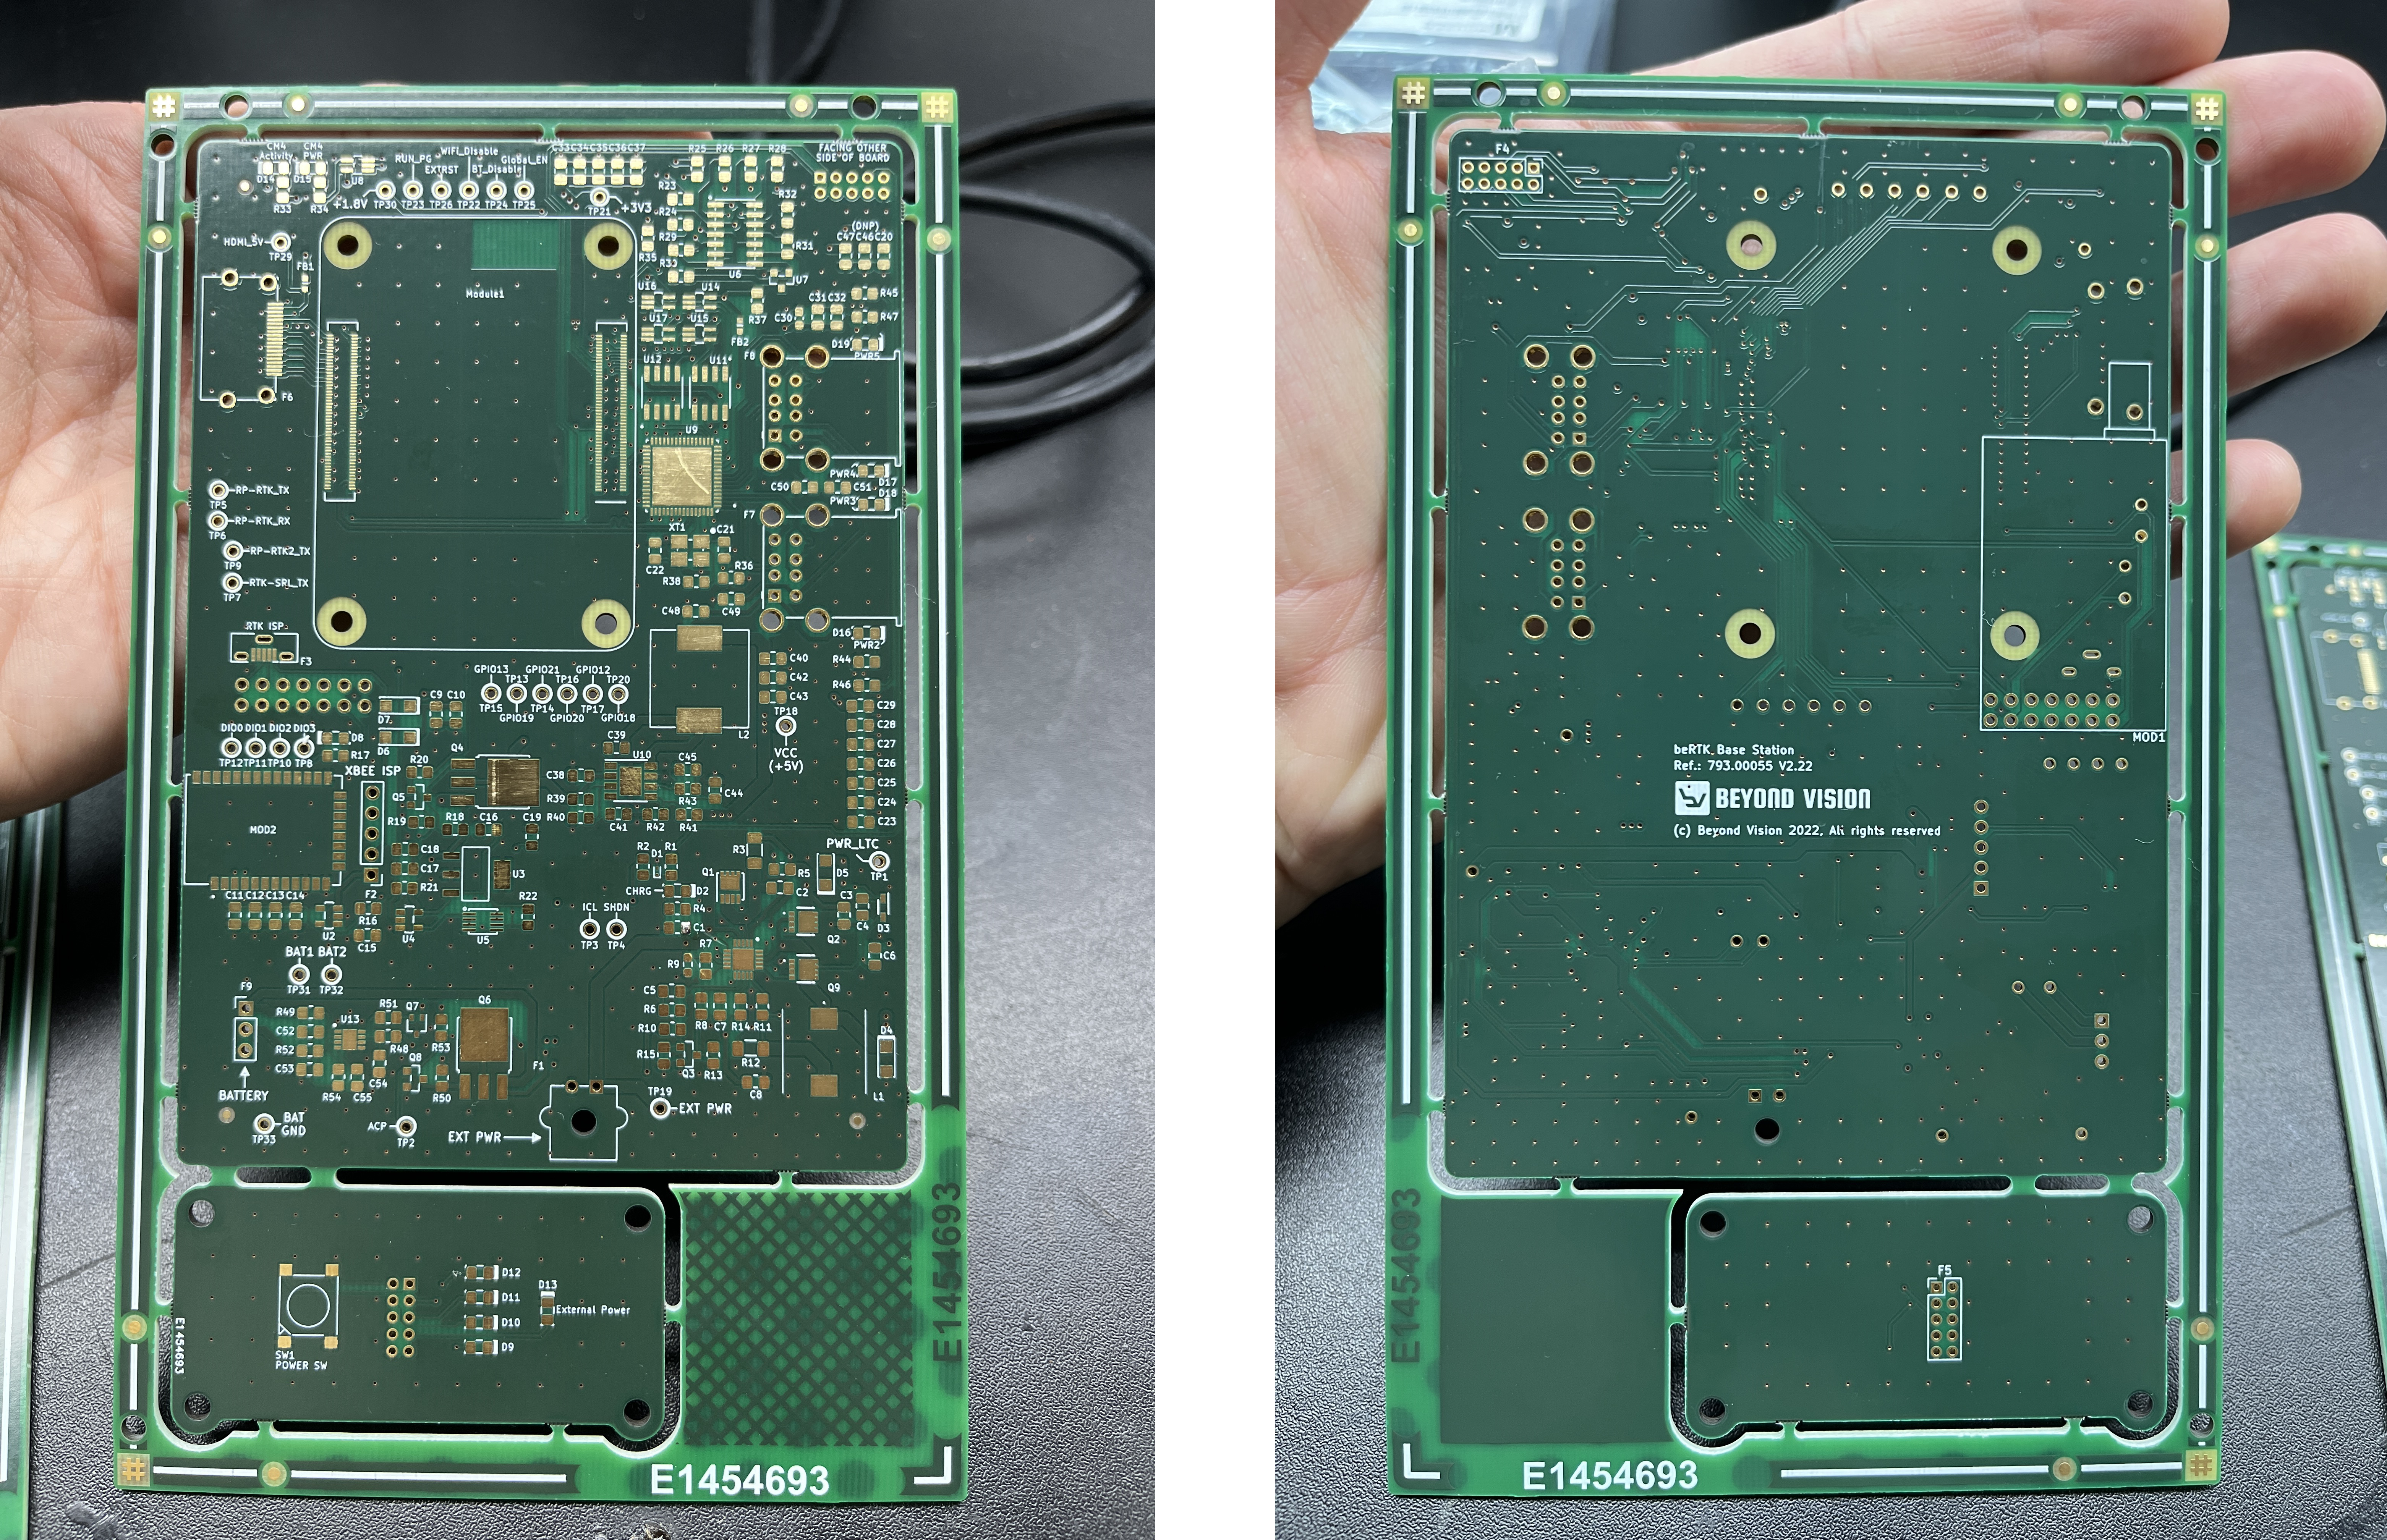
\includegraphics[width=1.0\textwidth]{Chapters/Figures/chapter5/prototype/1_proto_Front_Back_view.png}
	\caption{Front (left) and back (right) views of the new beRTK\textsuperscript{\textregistered} PCB.}
	\label{fig:1_proto_Front_Back_view}
\end{figure}% 1_proto_Front_Back_view

Having the manufactured PCB finally at hands (Figure~\ref{fig:1_proto_Front_Back_view}), the assembly process began by soldering the capacitors. This step proved itself to be very simple, due to the basic PCB hand soldering techniques needed, as well as to the nature of the components' footprints and packages selected, as mentioned in Section~\ref{sec:511_Placement}. Figure~\ref{fig:2_proto_Capacitors} shows the first capacitors soldered on the PCB.

\begin{figure}[h]
	\centering
	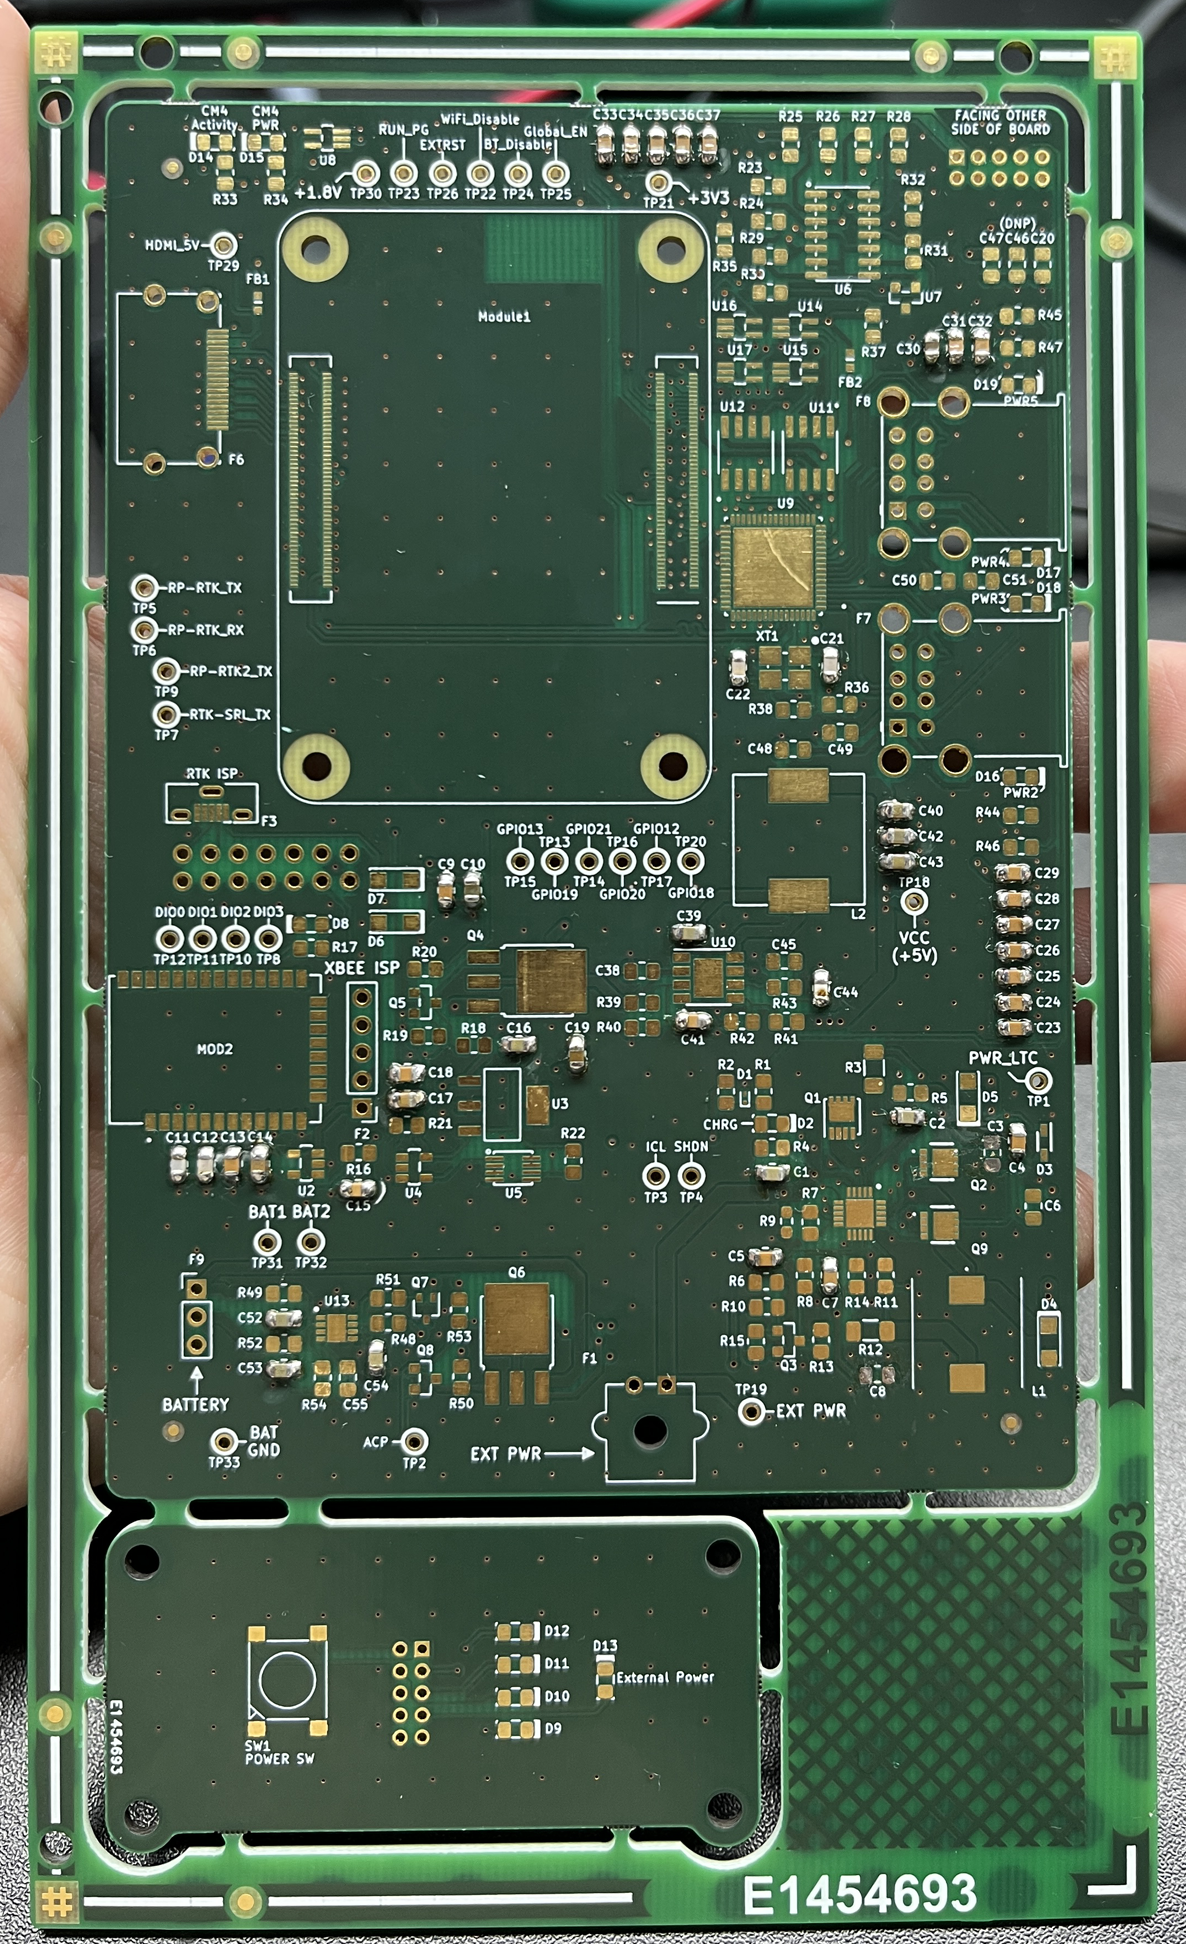
\includegraphics[width=0.5\textwidth]{Chapters/Figures/chapter5/prototype/2_proto_Capacitors.png}
	\caption{First components soldered.}
	\label{fig:2_proto_Capacitors}
\end{figure}% 2_proto_Capacitors

During the soldering process, the values for some components to solder suffered changes when compared to the schematics, due to the already available stock. This was, of course, accomplished whilst keeping in mind the values recommended to use by the datasheets used as reference. An example for such alteration regards the installation of the LTC4012 output capacitors -- represented by C3 and C8 in Figure~\ref{fig:LTC4012_circuit} -- suggested to be implemented as $20 \mu$F ceramic capacitors. Recalling Section~\ref{sec:3211_LTC4012}, it is assessed that~\cite{LTC4012} states that high-capacity ceramic capacitors worth $20 \mu$F or more are possible to use as the LTC4012's input and output capacitors. Therefore, $22 \mu$F ceramic capacitors rated at 50VDC are used in the prototype as both input and output capacitors for the battery charger's circuit. This is the same model used for the input and output capacitors, for the AP64501 buck converter's circuit (Figure~\ref{fig:AP64501_circuit}).

After soldering the capacitors, the second most-present components on the system were soldered: resistors. Just like the ``HandSolder'' version chosen for the capacitors footprints, the same was done for the footprints of every resistor with a 0805 package attributed. Also, similarly to what was done with the capacitors, some resistors' values were changed in order to fit the available stock. The most important change was made on the AP64501 circuit.
Originally, following the recommended component values for the typical AP64501 circuit presented in Table~\ref{tab:AP64501_recommended_values}, the necessary values for R41 and R42 (voltage divider to set the output voltage of the AP64501, Section~\ref{sec:3214_AP64501}) are specified at 115.8k$\Omega$ and 22.1k$\Omega$, respectively. However, this voltage divider can be accomplished with other resistor values, preferably with ones that would be available in stock, in order not to buy two single resistors specifically for this purpose. 

Since the AP64501 buck converter is a critical IC that sets up the entire 5V power supply, it is necessary that the resistance values chosen for the R41-R42 voltage divider allow the AP64501 to provide an output voltage value as close as possible to 5V. A range of 5V$\pm 5\%$, i.e. $[4.95,\, 5.05]$V was deemed reasonable. Recurring to expression (\ref{eq:R41_R42}), various R41-R42 combinations were taken into account to calculate the output voltage expected. Table~\ref{tab:R41_R42_values} compiles the best combinations found that fit the intended $\pm 5\%$ tolerance.

\begingroup
\begin{table}[H]
	\caption{Possible combinations and relative error for the R41-R42 voltage divider.}
	\label{tab:R41_R42_values}
	\centering%@{}l@{}@{}c@{}@{}c@{}@{}c@{}@{}c@{}
    % \setlength{\tabcolsep}{10pt} % Default value: 6pt
    % \renewcommand{\arraystretch}{1.5} % Default value: 1
	\begin{tabular}{cccc}
        \toprule
        \textbf{R41} \textbf{(k}$\mathbf{\Omega}$\textbf{)} & \textbf{R42} \textbf{(k}$\mathbf{\Omega}$\textbf{)} & $\mathbf{V_{OUT}}$ \textbf{(V)} & \textbf{Rel. error (\%)} \\
        \midrule
        124 & 24 & $4.933$ & $1.333$ \\
		\midrule
		390 & 75 & $4.960$ & $0.800$ \\
		\midrule
		270 & 51 & $5.0353$ & $0.706$ \\
		\midrule
		430 & 82 & $4.995$ & $0.098$ \\
        \bottomrule
    \end{tabular}
\end{table}
\endgroup

The relative error of the $V_{OUT}$ output voltage was determined for each combination, and the pair that presented the best results was R$41=430$k$\Omega$, R$42=82$k$\Omega$. These values allow the AP64501 to provide an output voltage of $4.995$V, which presents only a $0.098\%$ error, when compared to the expected 5V. Therefore, these were the R41 and R42 values soldered on the PCB.

% % ACRESCENTAR? --> programmed charge current do LTC4012: R3 era para ser 0.050R, eu meti 0.025R --> na altura dos testes, soldei dois 0.025R em serie para fazer os 0.050R; R12 era para ser 0.098R, eu meti 0.025R --> na altura dos testes, soldei quatro 0.025R em serie para fazer 0.1R, que é approx. 0.098R. --> se me perguntarem, sugerir meter isso no relatório. 
% R3 --> RCL, para fazer set up do input current limit feature.
% R12 --> -RSENSE, para programar a charge current.

% ACRESCENTAR? --> It should also be noted that, for the input resistors R11 and R14 of the LTC4012, 3k$\Omega$ resistors were used instead of the suggested $3.01$k$\Omega$. This was not a problem, since~\cite{LTC4012} informs that ``The LTC4012 operates best with 3.01k input resistors, although other resistors near this value can be used to accommodate standard sense resistor values.''.

%depois soldaram-se diodes, FB, ... dizer isto
After soldering capacitors and resistors, every other component was also assembled on the board, except the CM4. Some of these required special aid from a digital microscope -- shown in Figure~\ref{fig:3_proto_Microscope_Capacitors} --, and/or a rework station. The LAN9514 hub is an example of that. This IC's package presents (like others in the system) a large bottom pad that is not accessible with a regular PCB soldering iron, and therefore can only be soldered on the board using hot air. Its connecting pins are also very thin, and non-external to the package, which presents yet another disadvantage when it comes to hand soldering. Figure~\ref{fig:3_proto_ReworkStation} shows the rework station used, as well as a microscopic view of the soldering process for the LAN9514 hub.

\begin{figure}[h]
	\centering
	\includegraphics[width=0.5\textwidth]{Chapters/Figures/chapter5/prototype/3_proto_Microscope_Capacitors.png}
	\caption{Microscopic view of the soldering process.}
	\label{fig:3_proto_Microscope_Capacitors}
\end{figure}% 3_proto_Microscope_Capacitors

\begin{figure}[h]
	\centering
	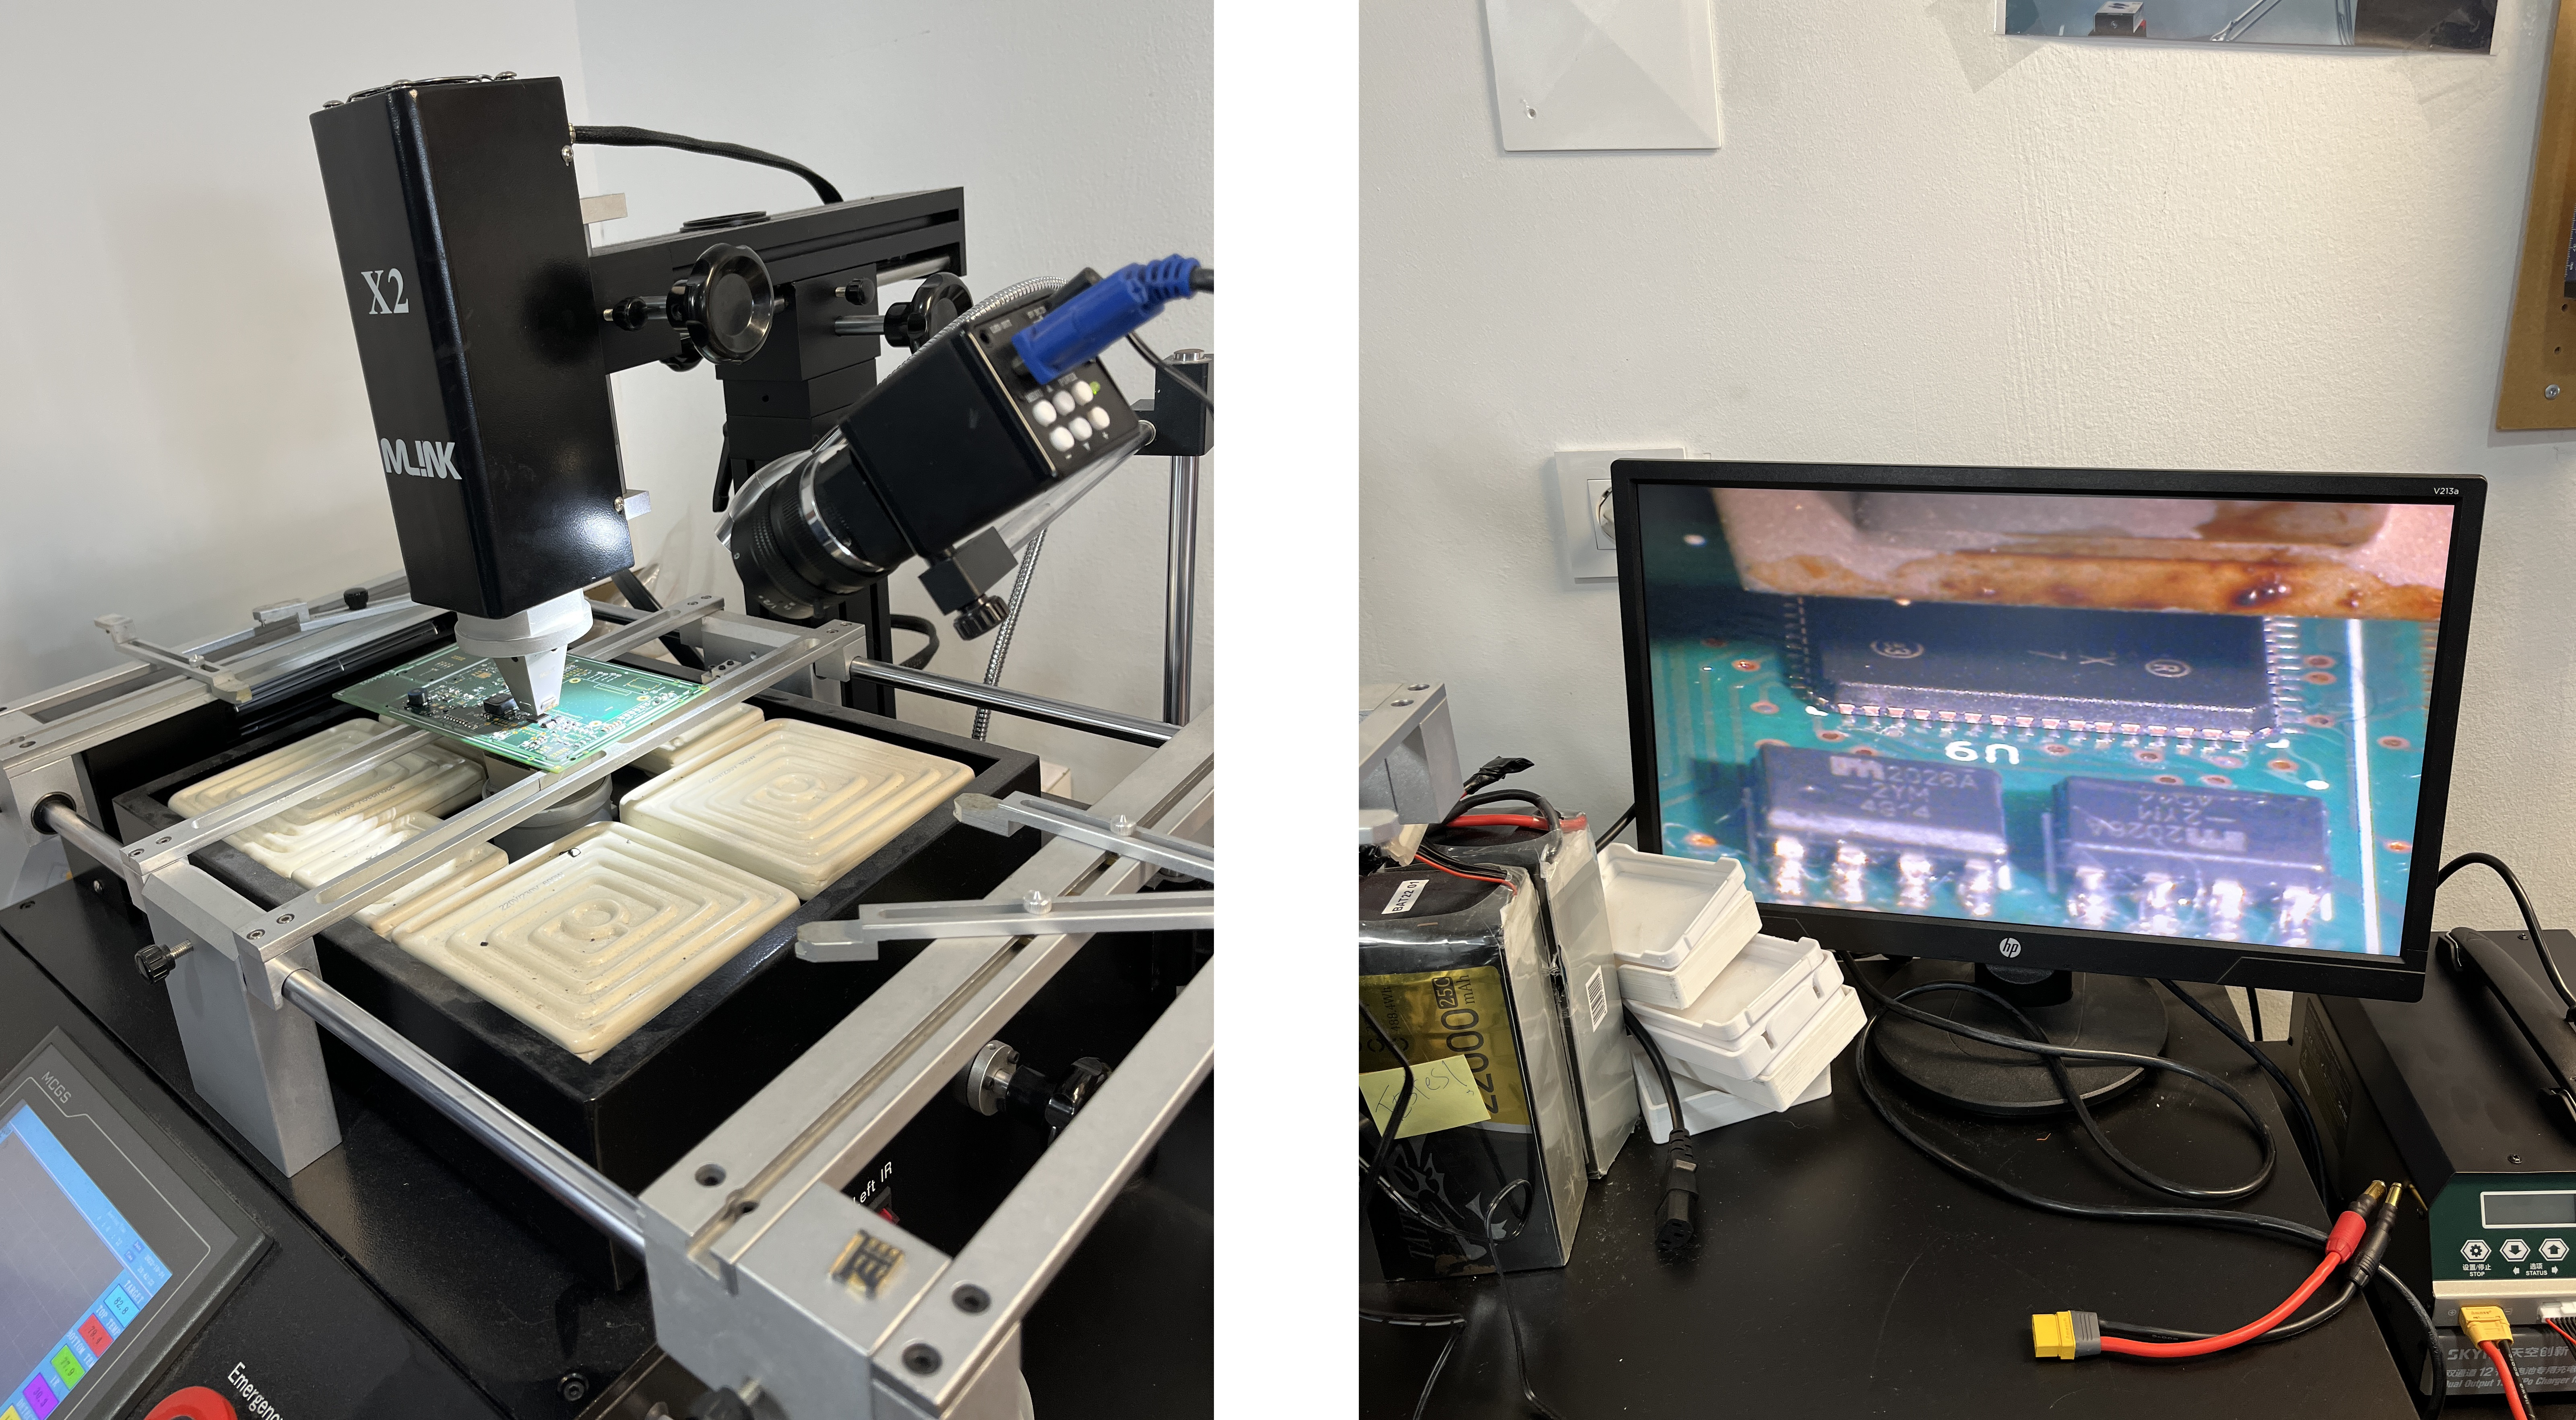
\includegraphics[width=1.0\textwidth]{Chapters/Figures/chapter5/prototype/3_proto_ReworkStation.png}
	\caption{Rework station used (left); microscopic view of the rework station's process (right).}
	\label{fig:3_proto_ReworkStation}
\end{figure}% 3_proto_ReworkStation

%falar dos indutores:
Regarding inductors, it must be mentioned that, even though the recommendations given by Table~\ref{tab:typ_inductor_values} point to an L1 inductor value $\geq 20 \mu$H for this project's case, the selection of this component was made relying on inequation (\ref{eq:L1}) instead, since it provides a more refined calculation for the inductor's value (i.e. it takes into account more variables that refer to the specific design). With this in mind, a $10 \mu$H inductor was chosen for L1, which is still greater than the $7.48 \mu$H determined by (\ref{eq:L1}). The DC current rating for this inductor was chosen to be 4A, providing a very safe margin.

As for the inductor L2, as stated in Section~\ref{sec:3214_AP64501}, an inductor value between $1 \mu$H to $10 \mu$H inductor should be selected, and it should have a DC current rating at least 35\% higher than the maximum 5A load current the AP64501 is able to output -- i.e. $6.75$A. Therefore, a $3.3 \mu$H inductor rated at 12.7A was selected for L2.

Ideally, all system's power supplies should be tested before assembling any module on the board, in order not to damage these valuable parts. This means double-checking the expected voltages in every important node of the system. In this case, the ZED-F9P and XBee modules were assembled prematurely (referring to this first testing phase).

% Programar a fonte para me dar a tensão que eu quero -- 15V @ 2A = rating de I do adapter
Having finished the assembly process, the prototype is ready for functional testing. Figure~\ref{fig:4_Soldering_finished} shows the final result of the assembly process, with an established connection to the external power connector.
Such connection originates from a DC power supply, which was used as the external power supply for the prototype.

\begin{figure}[h]
	\centering
	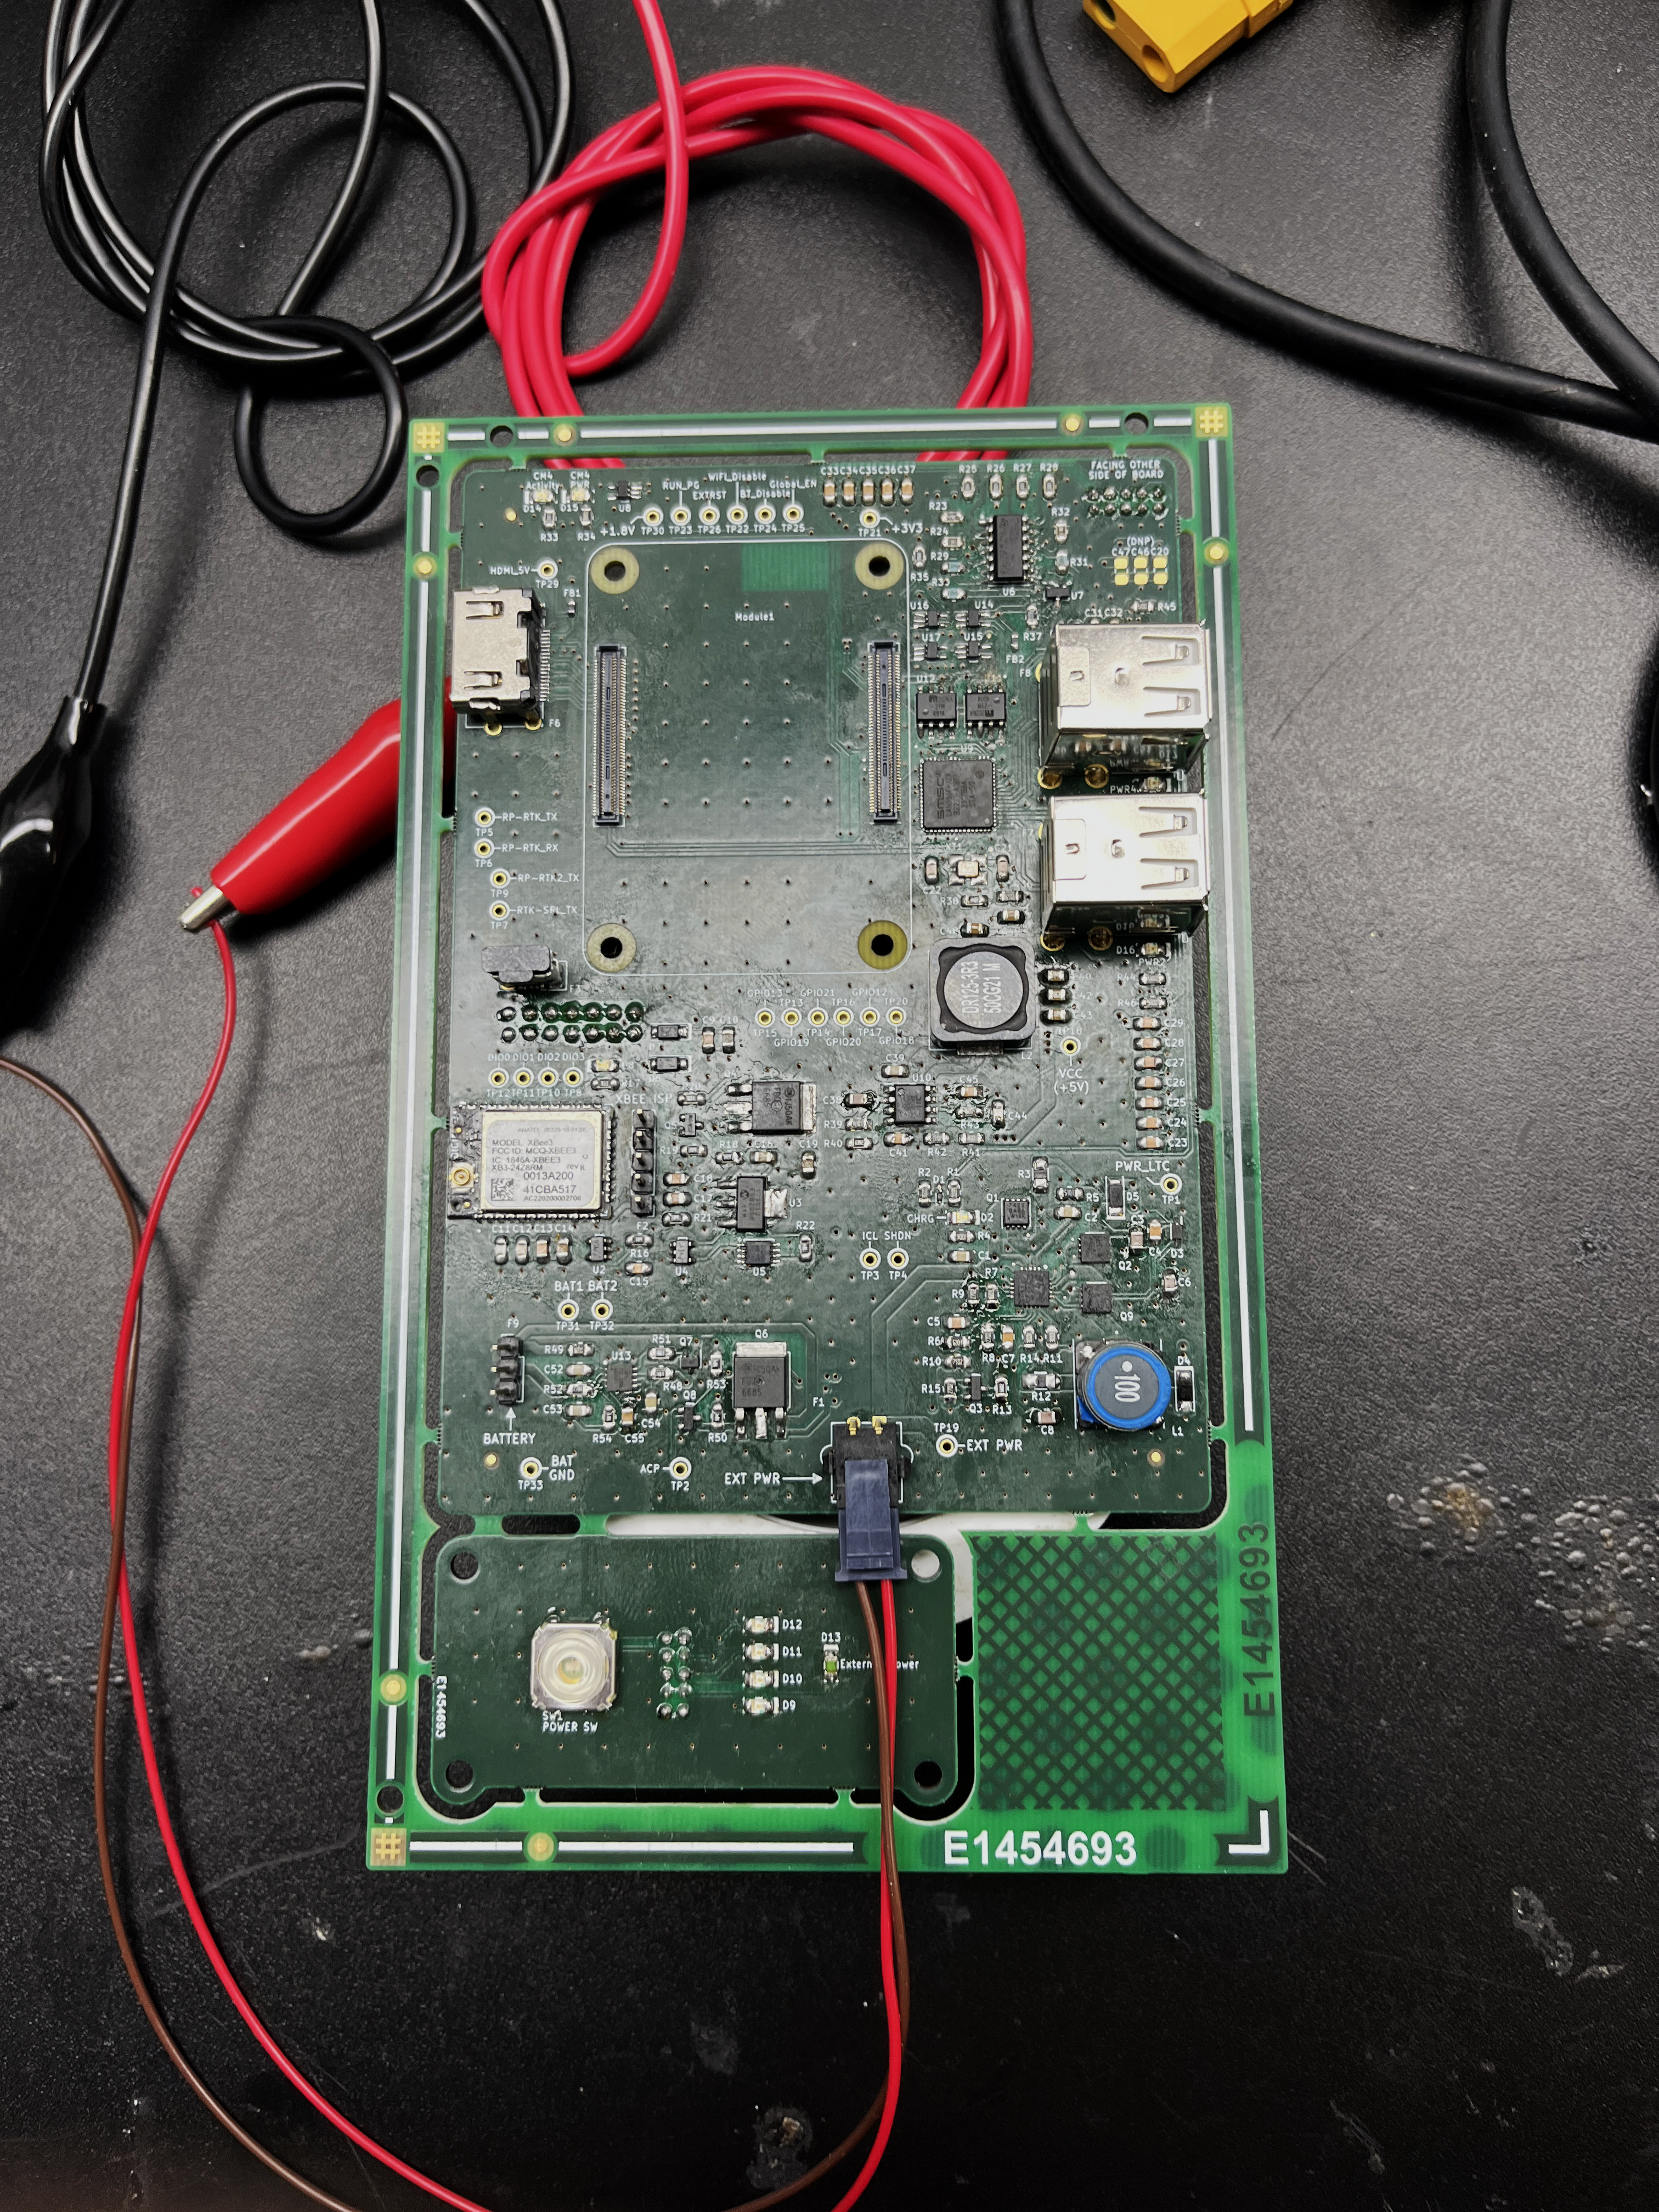
\includegraphics[width=0.6\textwidth]{Chapters/Figures/chapter5/prototype/4_Soldering_finished.png}
	\caption{Final result of the assembly process for the new beRTK\textsuperscript{\textregistered} PCB.}
	\label{fig:4_Soldering_finished}
\end{figure}% 4_Soldering_finished

% objetivo é Garantir que as tensões no circuito estão todas corretas (picar todos os pontos que se sabe que vão dar uma tensão fixa e ver se as tensões batem certo)
The functional tests are the first effective experiments the prototype is subject to. In this case, these tests occur at bench level and afterwards at field level, and are used to verify and analyse the device's relevant voltage levels, in order to evaluate its power supplies' basic functions. Functional testing is critical, since the following performance-related tests dictate the device's limitations, and can only take place once all the intended functionalities have been extensively checked. If applicable, a final testing category, related to certification, double-checks the device's operation in order to assess its compliance to applicable European norms.

% 3. Antes de ligar a fonte (vou trabalhar com a mais pequena): a primeira vez que ligar, garantir que quando se liga, estar atento se alguma coisa larga fumo e tocar na placa para sentir se está a ficar muito quente;
To start the functional tests, it must first be verified if the prototype is able to support the intended external power from the DC supply. This equipment was adjusted in order to first supply 12VDC, at a maximum continuous current of 1.00A, in order to verify if there was any component overheat/burnout. Since there were no such problems, the supply was once again adjusted, this time up to 15VDC, and the maximum continuous current was increased to 2.00A, corresponding to the rating of the external DC adapter considered, as mentioned in Section~\ref{sec:3211_LTC4012}.

The device was tested considering its three possible power modes:
\begin{enumerate}
	\item External power ON, backup battery OFF -- Figure~\ref{fig:5_proto_first_test_ONLY_EXT_PWR};
	\item Backup battery ON, external power OFF -- Figure~\ref{fig:5_proto_first_test_ONLY_Batteries};
	\item External power ON, backup battery ON -- Figure~\ref{fig:5_proto_first_test_EXT_ON_Batteries}.
\end{enumerate}

\begin{figure}[h]
	\centering
	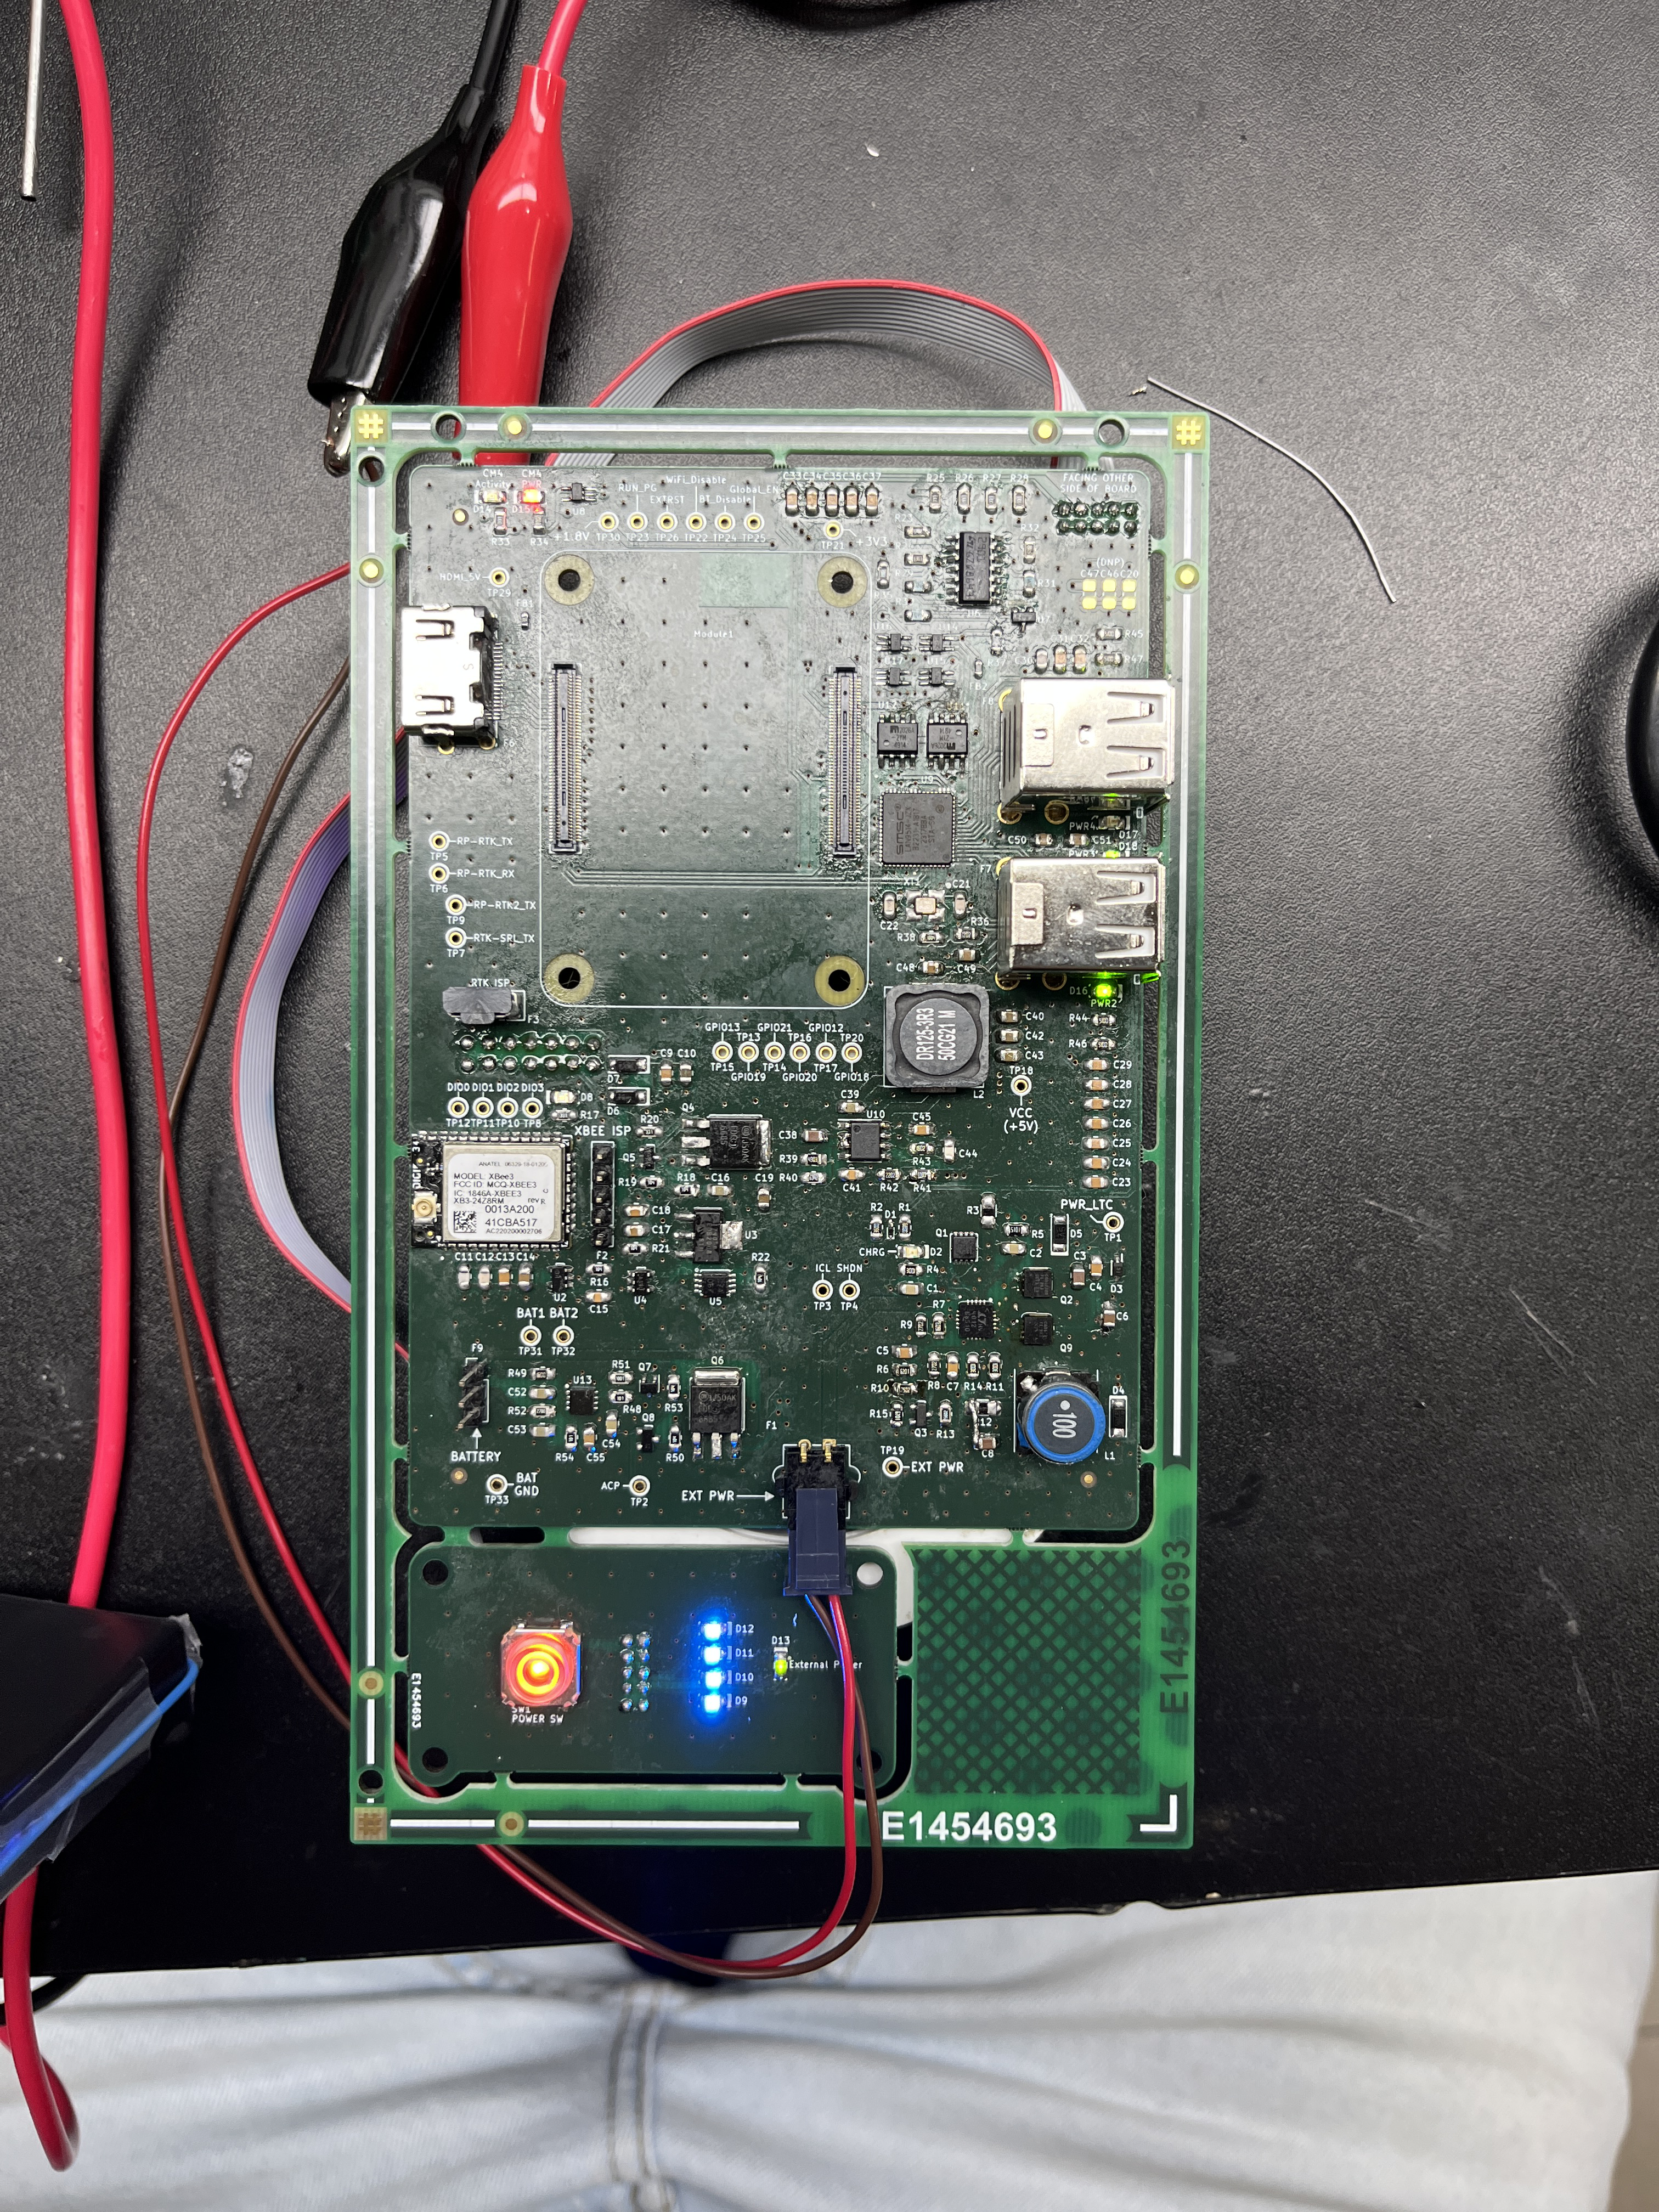
\includegraphics[width=0.7\textwidth]{Chapters/Figures/chapter5/prototype/5_proto_first_test_ONLY_EXT_PWR.png}
	\caption{Functional testing of the new beRTK\textsuperscript{\textregistered} PCB (external power only; without the Raspberry Pi CM4).}
	\label{fig:5_proto_first_test_ONLY_EXT_PWR}
\end{figure}% 5_proto_first_test_ONLY_EXT_PWR

\begin{figure}[h]
	\centering
	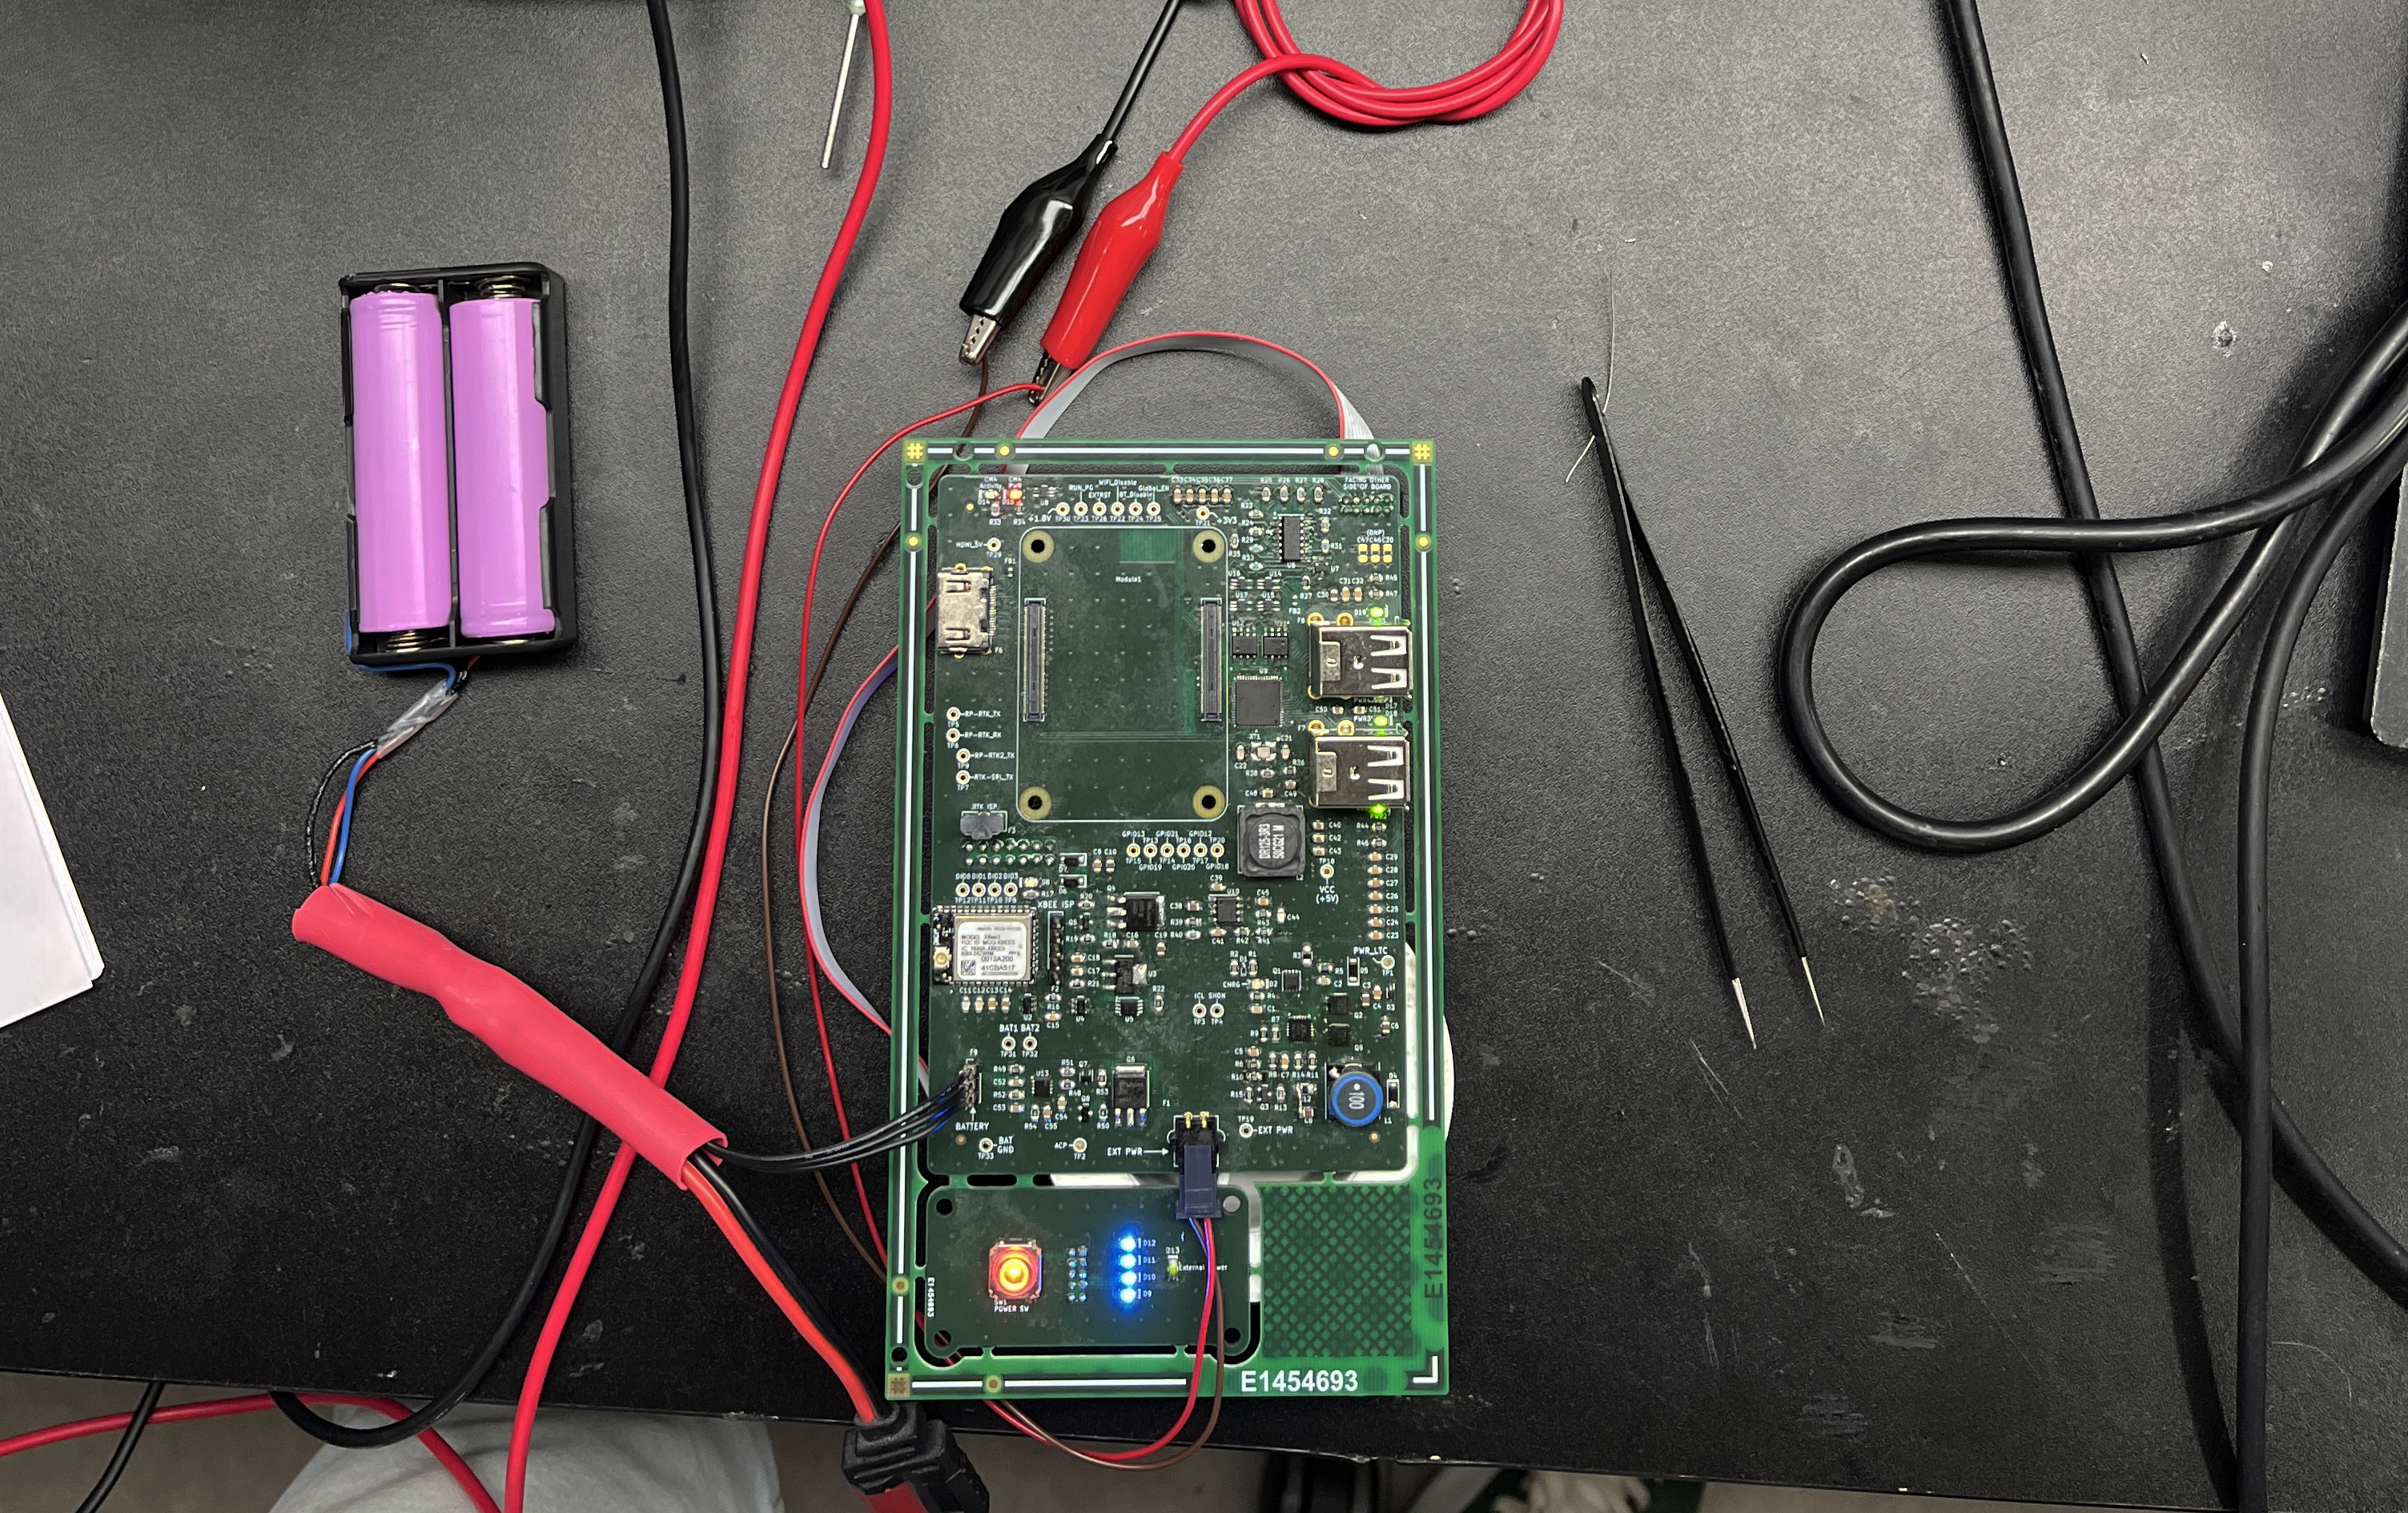
\includegraphics[width=1.0\textwidth]{Chapters/Figures/chapter5/prototype/5_proto_first_test_ONLY_Batteries.png}
	\caption{Functional testing of the new beRTK\textsuperscript{\textregistered} PCB (battery pack power only; without the Raspberry Pi CM4).}
	\label{fig:5_proto_first_test_ONLY_Batteries}
\end{figure}% 5_proto_first_test_ONLY_Batteries

\begin{figure}[h]
	\centering
	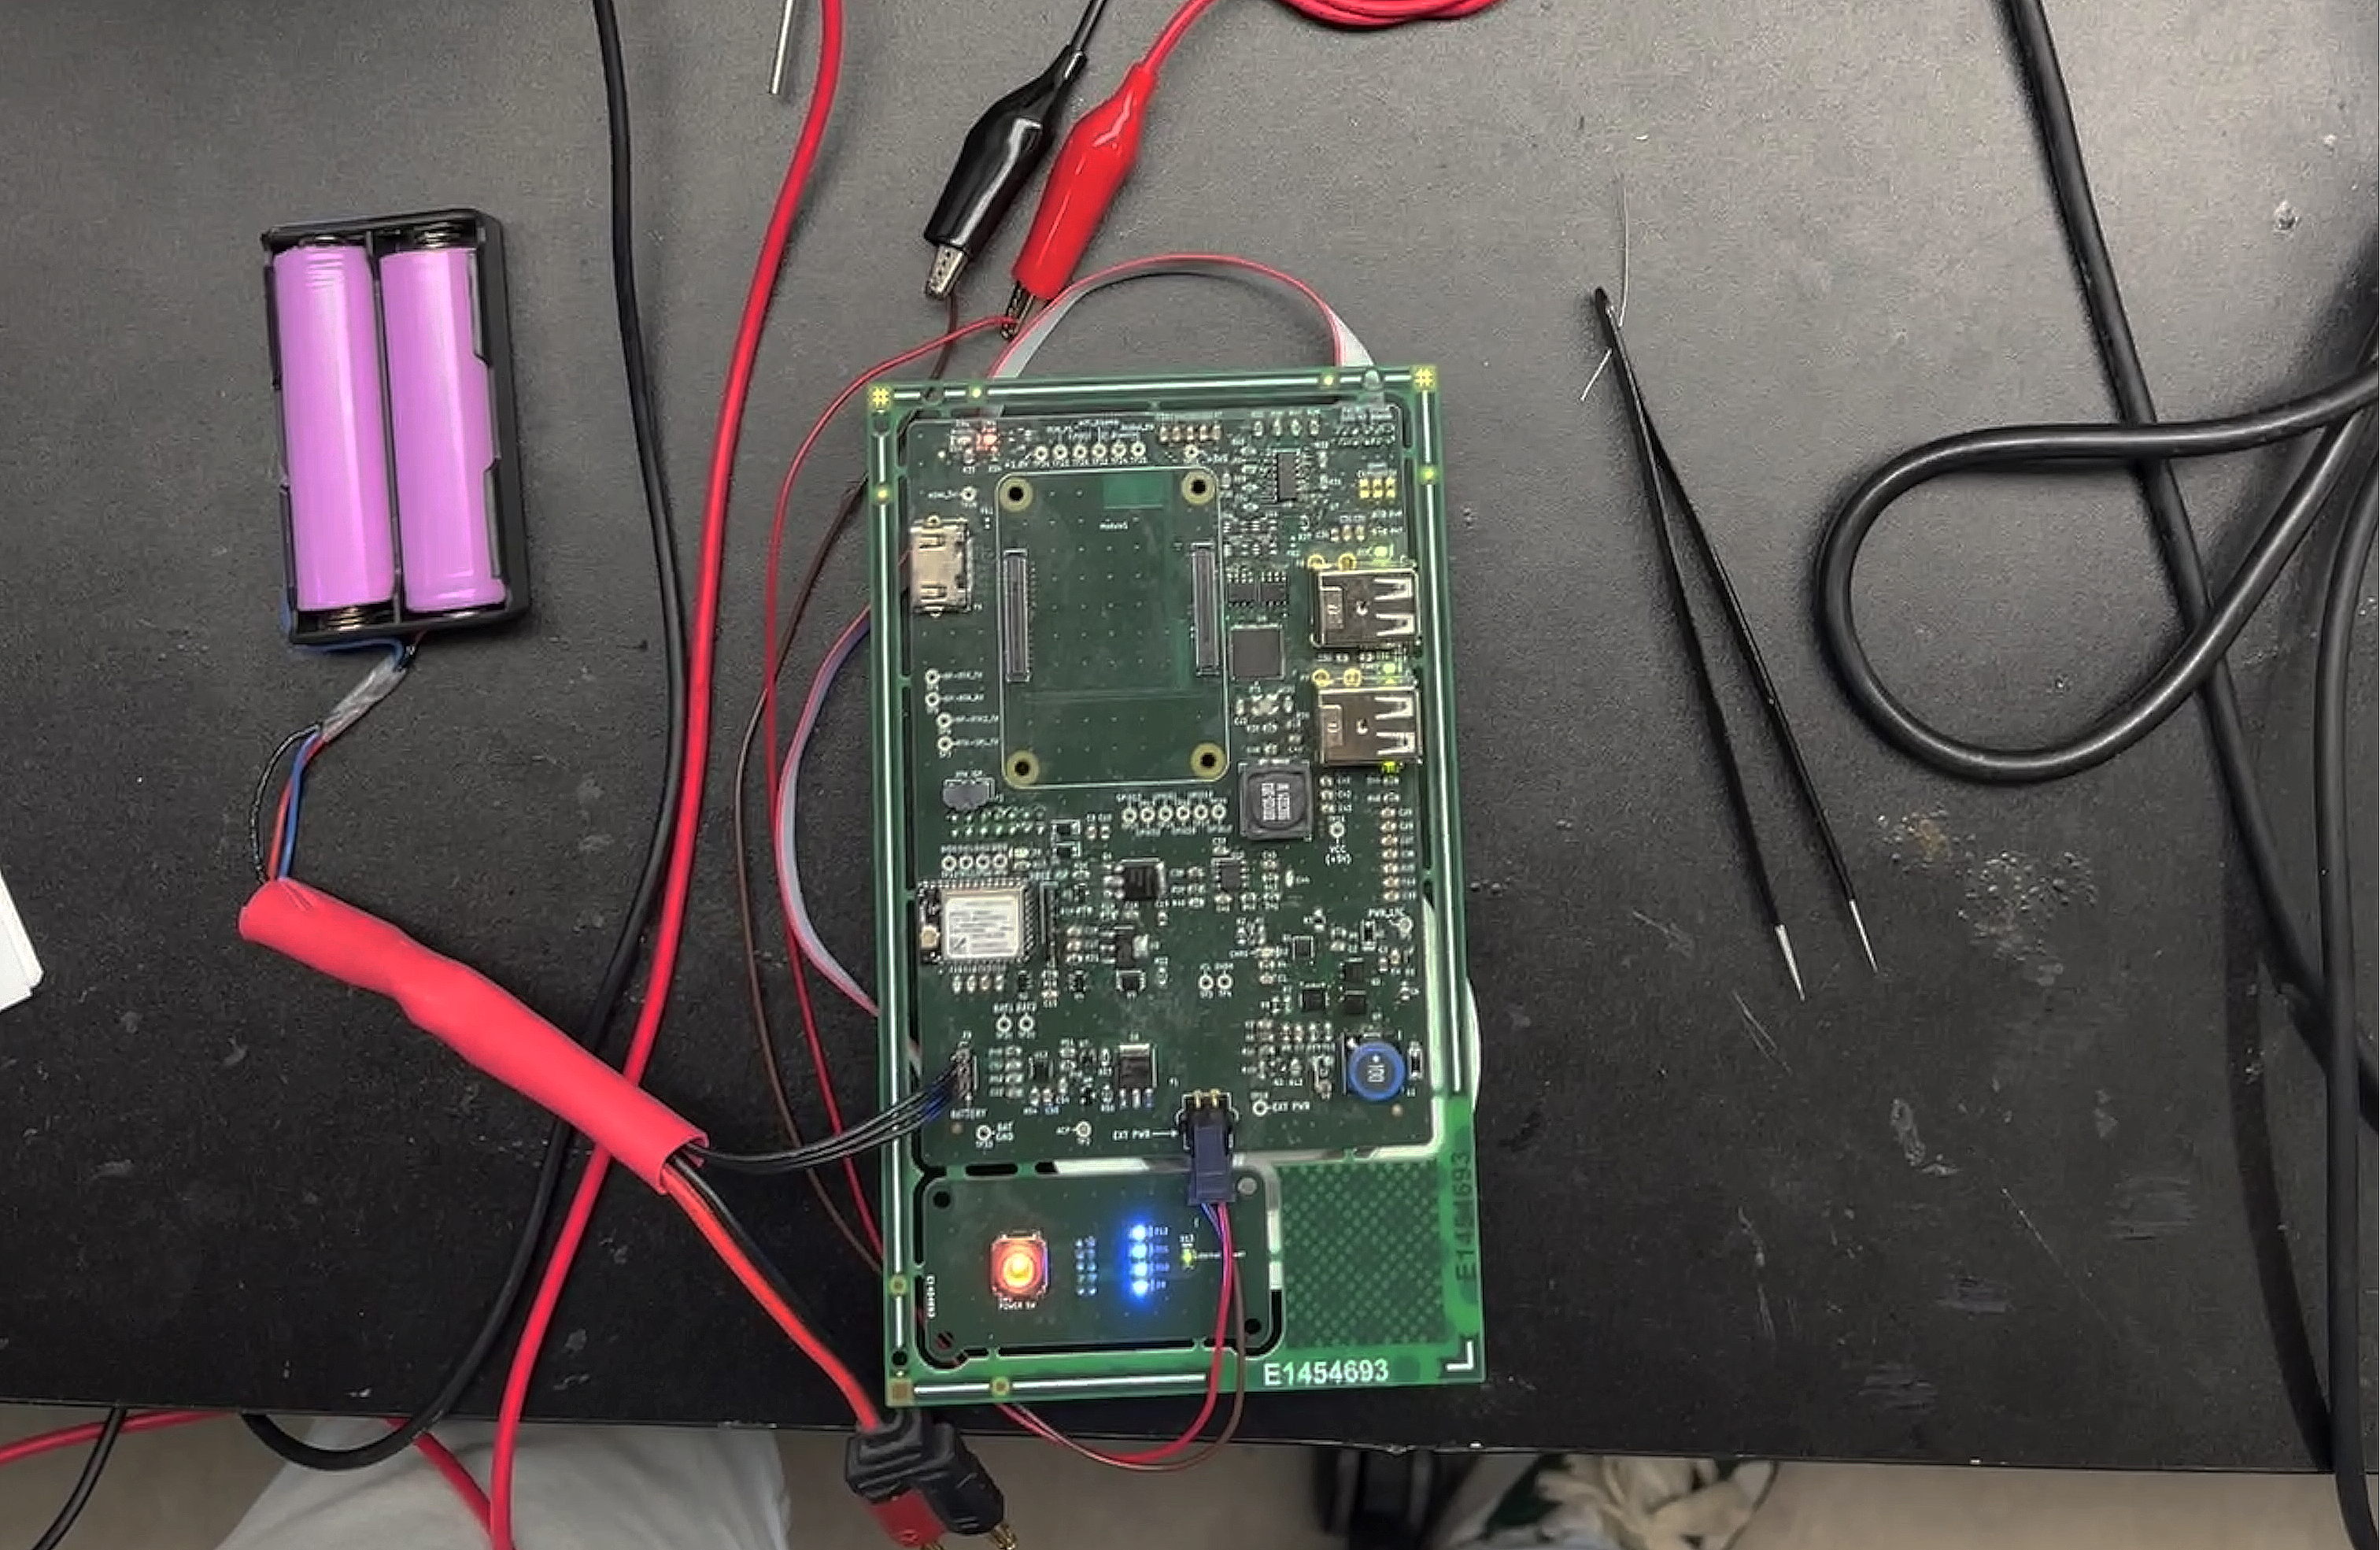
\includegraphics[width=1.0\textwidth]{Chapters/Figures/chapter5/prototype/5_proto_first_test_EXT_ON_Batteries.png}
	\caption{Functional testing of the new beRTK\textsuperscript{\textregistered} PCB (external power and battery pack power applied; without the Raspberry Pi CM4).}
	\label{fig:5_proto_first_test_EXT_ON_Batteries}
\end{figure}% 5_proto_first_test_EXT_ON_Batteries


%ssSssSssSssSssSssSssSssSssSssSssSssSssSssSssSssSssSssSssSssSssSssSssSssSssSssS
\subsubsection{CM4 Unmounted from the Prototype}\label{sec:5331_CM4_UNmounted}

The functional tests were first run without the CM4 mounted on the prototype -- as it is possible to observe through Figures~\ref{fig:5_proto_first_test_ONLY_EXT_PWR},~\ref{fig:5_proto_first_test_ONLY_Batteries} and~\ref{fig:5_proto_first_test_EXT_ON_Batteries} --, in order not to damage this module in case of unexpected levels. It must also be noted that all voltages were measured using the BAT\_GND test point, which is connected to the general GND layer.


\begingroup
\begin{table}[H]
	\caption{LTC4012 circuit's most relevant voltages expected and measured, for all operational modes, with the CM4 unmounted from the prototype.}
	\label{tab:LTC4012_3_modes_NO_CM4}
	\centering
	\resizebox{\textwidth}{!}{%
	\begin{tabular}{lcccccc}
        \toprule
		\multicolumn{7}{c}{\textbf{LTC4012 Circuit (CM4 unmounted from the board)}} \\
		\midrule
        {} & \multicolumn{2}{c}{\textbf{Mode 1}} & \multicolumn{2}{c}{\textbf{Mode 2}} & \multicolumn{2}{c}{\textbf{Mode 3}} \\
		\midrule
		{} & \textbf{Exp. (V)} & \textbf{Meas. (V)} & \textbf{Exp. (V)} & \textbf{Meas. (V)} & \textbf{Exp. (V)} & \textbf{Meas. (V)} \\
		\midrule
		\textbf{EXT\_PWR} & $15.00$ & $15.05$ & $0.00$  & $0.00$  & $15.00$ & $15.05$ \\
        \midrule
		\textbf{PWR\_LTC} & $15.00$ & $15.08$ & $8.40$  & $8.43$  & $15.00$ & $15.08$ \\
        \midrule
		\textbf{VBAT} 	  & $8.37$  & $8.36$  & $8.40$  & $8.15$  & $8.40$  & $8.13$ \\
        \midrule
		\textbf{!ACP} 	  & $0.00$  & $0.09$  & $5.00$  & $4.96$  & $0.00$  & $0.09$ \\
        \midrule
		% \textbf{SW} 	  & $0.00$  & $0.00$  & $0.00$  & $0.00$  & $0.00$  & $0.00$ \\
        % \midrule
		% \textbf{INTVDD}   & $0.00$  & $0.00$  & $0.00$  & $0.00$  & $0.00$  & $0.00$ \\
        % \midrule
		% \textbf{FBDIV}    & $0.00$  & $0.00$  & $0.00$  & $0.00$  & $0.00$  & $0.00$ \\
        % \midrule % so é interessante caso esteja a haver carga de baterias
		\textbf{VFB} 	  & $1.21$  & $1.21$  & $1.21$  & $1.20$  & $1.21$  & $1.21$ \\
        % \midrule
		% \textbf{PROG} 	  & $1.21$  & $0.54$  & $0.00$  & $0.00$  & $0.00$  & $0.00$ \\
        \bottomrule
    \end{tabular}}
\end{table}
\endgroup% LTC4012 Circuit

Table~\ref{tab:LTC4012_3_modes_NO_CM4} verifies a VBAT voltage of 8.37V in Mode 1. This voltage is programmed through the voltage divider composed by resistors R7 and R9, and can be calculated using equation (\ref{eq:v_bat}), as explained in Section~\ref{sec:3211_LTC4012}. These resistors are suggested to be equal to 169k$\Omega$ and $28.4$k$\Omega$ (respectively), according to~\cite{LTC4012}, however, using this same equation and selecting the more well-suited available resistors, these were selected as R$7=160$k$\Omega$ and R$9=27$k$\Omega$, resulting in the $VBAT=8.369 \approx 8.37$V value measured.


\begingroup
\begin{table}[H]
	\caption{BQ29209 circuit's most relevant voltages expected and measured, for all operational modes, with the CM4 unmounted from the prototype.}
	\label{tab:BQ29209_3_modes_NO_CM4}
	\centering
	\resizebox{\textwidth}{!}{%
	\begin{tabular}{lcccccc}
        \toprule
		\multicolumn{7}{c}{\textbf{BQ29209 Circuit (CM4 unmounted from the board)}} \\
		\midrule
        {} & \multicolumn{2}{c}{\textbf{Mode 1}} & \multicolumn{2}{c}{\textbf{Mode 2}} & \multicolumn{2}{c}{\textbf{Mode 3}} \\
		\midrule
		{} & \textbf{Exp. (V)} & \textbf{Meas. (V)} & \textbf{Exp. (V)} & \textbf{Meas. (V)} & \textbf{Exp. (V)} & \textbf{Meas. (V)} \\
		\midrule
		\textbf{VBAT} 		& $8.37$ & $8.36$ & $8.40$ & $8.15$ & $8.40$ & $8.13$ \\
        \midrule
		\textbf{BAT1-BAT2} 	& $0.00$ & $0.00$ & $4.20$ & $4.07$ & $4.20$ & $4.07$ \\
        \midrule
		\textbf{BAT2} 		& $0.00$ & $0.00$ & $4.20$ & $4.08$ & $4.20$ & $4.08$ \\
        \midrule
		\textbf{VBAT\_STAT} & $0.00$ & $8.11$ & $8.40$ & $7.87$ & $8.40$ & $7.90$ \\
        \bottomrule
    \end{tabular}}
\end{table}
\endgroup% BQ29209 Circuit

%explicar os resultados da tabela do BQ29209
When observing Figure~\ref{fig:5_proto_first_test_ONLY_EXT_PWR}, an undesired occurrence can be seen. The status LEDs are lit up when Mode 1 is in operation.
Such event should not happen, since the status LEDs are used only to indicate the battery pack's status, and should be off when only external power is plugged in to feed the system.
Referring back to tables~\ref{tab:LTC4012_3_modes_NO_CM4} and~\ref{tab:BQ29209_3_modes_NO_CM4}, it can be concluded that the VBAT net will never measure a voltage value anywhere close to zero, due to the programming done for the VBAT voltage on the LTC4012 charger, as explained earlier. This reveals to be a problem when Mode 1 is chosen. This problem is related to the clash between the voltage on the !ACP pin and the 5V net (referring back to Figure~\ref{fig:LTC4012_circuit}). These are the reasons why all the status voltage LEDs turn on while Mode 1 is in operation and should be worked on in the future. 


\begingroup
\begin{table}[H]
	\caption{Power switch circuit's most relevant voltages expected and measured, for all operational modes, with the CM4 unmounted from the prototype.}
	\label{tab:PowerSwitch_3_modes_NO_CM4}
	\centering
	\resizebox{\textwidth}{!}{%
	\begin{tabular}{lcccccc}
        \toprule
		\multicolumn{7}{c}{\textbf{Power Switch Circuit (CM4 unmounted from the board)}} \\
		\midrule
        {} & \multicolumn{2}{c}{\textbf{Mode 1}} & \multicolumn{2}{c}{\textbf{Mode 2}} & \multicolumn{2}{c}{\textbf{Mode 3}} \\
		\midrule
		{} & \textbf{Exp. (V)} & \textbf{Meas. (V)} & \textbf{Exp. (V)} & \textbf{Meas. (V)} & \textbf{Exp. (V)} & \textbf{Meas. (V)} \\
		\midrule
		\textbf{PWR\_AP64501} 	& $15.00$ & $14.93$ & $8.40$  & $8.31$  & $15.00$ & $14.94$ \\
        \midrule
		\textbf{PWR\_LED} 		& $5.00$  & $4.94$  & $5.00$  & $4.95$  & $5.00$  & $4.94$ \\
        \bottomrule
    \end{tabular}}
\end{table}
\endgroup% Power Switch Circuit


\begingroup
\begin{table}[H]
	\caption{AP64501 circuit's most relevant voltages expected and measured, for all operational modes, with the CM4 unmounted from the prototype.}
	\label{tab:AP64501_3_modes_NO_CM4}
	\centering
	\resizebox{\textwidth}{!}{%
	\begin{tabular}{lcccccc}
        \toprule
		\multicolumn{7}{c}{\textbf{AP64501 Circuit (CM4 unmounted from the board)}} \\
		\midrule
        {} & \multicolumn{2}{c}{\textbf{Mode 1}} & \multicolumn{2}{c}{\textbf{Mode 2}} & \multicolumn{2}{c}{\textbf{Mode 3}} \\
		\midrule
		{} & \textbf{Exp. (V)} & \textbf{Meas. (V)} & \textbf{Exp. (V)} & \textbf{Meas. (V)} & \textbf{Exp. (V)} & \textbf{Meas. (V)} \\
		\midrule
		\textbf{PWR\_AP64501} 	& $15.00$ & $14.93$ & $8.40$  & $8.31$  & $15.00$ & $14.94$ \\
        \midrule
		\textbf{VCC (+5V)} 		& $5.00$  & $5.01$  & $5.00$  & $5.01$  & $5.00$  & $5.01$ \\
        \midrule
		\textbf{EN}				& $2.96$  & $2.94$ 	& $1.66$  & $1.64$  & $2.96$  & $2.94$ \\
        % \midrule
		% \textbf{FB} 			& $00.00$ & $00.00$ & $00.00$ & $00.00$ & $00.00$ & $00.00$ \\
        \bottomrule
    \end{tabular}}
\end{table}
\endgroup% AP64501 Circuit

Tables~\ref{tab:PowerSwitch_3_modes_NO_CM4} and~\ref{tab:AP64501_3_modes_NO_CM4} reveal the correct operation of the power switch circuit and AP64501 buck converter. In practical terms, the power switch circuit corresponds to whether the input power voltage from either the external adapter or the battery pack is allowed into the input terminal of the AP64501 (PWR\_AP64501), as mentioned in Section~\ref{sec:3213_SWITCH}. The correct workings of both circuits are related to the lighting status of the switch's (SW1) integrated LED (PWR\_LED, present in the HMI circuit), followed by the 5V output from the AP64501 (VCC (+5V)).





%ssSssSssSssSssSssSssSssSssSssSssSssSssSssSssSssSssSssSssSssSssSssSssSssSssSssS
\subsubsection{CM4 Mounted on the Prototype}\label{5332_CM4_Mounted_ON}

After verifying the voltage levels were stable and indicated for the CM4, the module was assembled on the board's respective connectors, and the same functional tests as exposed in Section~\ref{sec:5331_CM4_UNmounted} were conducted.

Assembling the module on the board enables the 3.3V net. Since the only IC that uses this supply is the LAN9514 hub, the measured voltages for every other circuit should remain unaltered.

\begingroup
\begin{table}[H]
	\caption{LTC4012 circuit's most relevant voltages expected and measured, for all operational modes, with the CM4 mounted on the prototype.}
	\label{tab:LTC4012_3_modes_WITH_CM4}
	\centering
	\resizebox{\textwidth}{!}{%
	\begin{tabular}{lcccccc}
        \toprule
		\multicolumn{7}{c}{\textbf{LTC4012 Circuit (CM4 mounted on the board)}} \\
		\midrule
        {} & \multicolumn{2}{c}{\textbf{Mode 1}} & \multicolumn{2}{c}{\textbf{Mode 2}} & \multicolumn{2}{c}{\textbf{Mode 3}} \\
		\midrule
		{} & \textbf{Exp. (V)} & \textbf{Meas. (V)} & \textbf{Exp. (V)} & \textbf{Meas. (V)} & \textbf{Exp. (V)} & \textbf{Meas. (V)} \\
		\midrule
		\textbf{EXT\_PWR} & $15.00$ & $15.05$ & $0.00$  & $0.00$  & $15.00$ & $15.05$ \\
        \midrule
		\textbf{PWR\_LTC} & $15.00$ & $15.07$ & $8.40$  & $8.42$  & $15.00$ & $15.07$ \\
        \midrule
		\textbf{VBAT} 	  & $8.37$  & $8.35$  & $8.40$  & $8.13$  & $8.40$  & $8.12$ \\
        \midrule
		\textbf{!ACP} 	  & $0.00$  & $0.09$  & $5.00$  & $4.97$  & $0.00$  & $0.09$ \\
        \midrule
		% \textbf{SW} 	  & $0.00$  & $0.00$  & $0.00$  & $0.00$  & $0.00$  & $0.00$ \\
        % \midrule
		% \textbf{INTVDD}   & $0.00$  & $0.00$  & $0.00$  & $0.00$  & $0.00$  & $0.00$ \\
        % \midrule
		% \textbf{FBDIV}    & $0.00$  & $0.00$  & $0.00$  & $0.00$  & $0.00$  & $0.00$ \\
        % \midrule % so é interessante caso esteja a haver carga de baterias
		\textbf{VFB} 	  & $1.21$  & $1.21$  & $1.21$  & $1.20$  & $1.21$  & $1.21$ \\
        % \midrule
		% \textbf{PROG} 	  & $1.21$  & $0.54$  & $0.00$  & $0.00$  & $0.00$  & $0.00$ \\
        \bottomrule
    \end{tabular}}
\end{table}
\endgroup% LTC4012_3_modes_WITH_CM4

\begingroup
\begin{table}[H]
	\caption{BQ29209 circuit's most relevant voltages expected and measured, for all operational modes, with the CM4 mounted on the prototype.}
	\label{tab:BQ29209_3_modes_WITH_CM4}
	\centering
	\resizebox{\textwidth}{!}{%
	\begin{tabular}{lcccccc}
        \toprule
		\multicolumn{7}{c}{\textbf{BQ29209 Circuit (CM4 mounted on the board)}} \\
		\midrule
        {} & \multicolumn{2}{c}{\textbf{Mode 1}} & \multicolumn{2}{c}{\textbf{Mode 2}} & \multicolumn{2}{c}{\textbf{Mode 3}} \\
		\midrule
		{} & \textbf{Exp. (V)} & \textbf{Meas. (V)} & \textbf{Exp. (V)} & \textbf{Meas. (V)} & \textbf{Exp. (V)} & \textbf{Meas. (V)} \\
		\midrule
		\textbf{VBAT} 		& $8.37$ & $8.35$ & $8.40$ & $8.13$ & $8.40$ & $8.12$ \\
        \midrule
		\textbf{BAT1-BAT2} 	& $0.00$ & $0.00$ & $4.20$ & $4.05$ & $4.20$ & $4.05$ \\
        \midrule
		\textbf{BAT2} 		& $0.00$ & $0.00$ & $4.20$ & $4.08$ & $4.20$ & $4.08$ \\
        \midrule
		\textbf{VBAT\_STAT} & $0.00$ & $8.10$ & $8.40$ & $7.84$ & $8.40$ & $7.88$ \\
        \bottomrule
    \end{tabular}}
\end{table}
\endgroup% BQ29209_3_modes_WITH_CM4

\begingroup
\begin{table}[H]
	\caption{Power switch circuit's most relevant voltages expected and measured, for all operational modes, with the CM4 mounted on the prototype.}
	\label{tab:PowerSwitch_3_modes_WITH_CM4}
	\centering
	\resizebox{\textwidth}{!}{%
	\begin{tabular}{lcccccc}
        \toprule
		\multicolumn{7}{c}{\textbf{Power Switch Circuit (CM4 mounted on the board)}} \\
		\midrule
        {} & \multicolumn{2}{c}{\textbf{Mode 1}} & \multicolumn{2}{c}{\textbf{Mode 2}} & \multicolumn{2}{c}{\textbf{Mode 3}} \\
		\midrule
		{} & \textbf{Exp. (V)} & \textbf{Meas. (V)} & \textbf{Exp. (V)} & \textbf{Meas. (V)} & \textbf{Exp. (V)} & \textbf{Meas. (V)} \\
		\midrule
		\textbf{PWR\_AP64501} 	& $15.00$ & $14.93$ & $8.40$  & $8.27$  & $15.00$ & $14.94$ \\
        \midrule
		\textbf{PWR\_LED} 		& $5.00$  & $4.94$  & $5.00$  & $4.95$  & $5.00$  & $4.94$ \\
        \bottomrule
    \end{tabular}}
\end{table}
\endgroup% PowerSwitch_3_modes_WITH_CM4

\begingroup
\begin{table}[H]
	\caption{AP64501 circuit's most relevant voltages expected and measured, for all operational modes, with the CM4 mounted on the prototype.}
	\label{tab:AP64501_3_modes_WITH_CM4}
	\centering
	\resizebox{\textwidth}{!}{%
	\begin{tabular}{lcccccc}
        \toprule
		\multicolumn{7}{c}{\textbf{AP64501 Circuit (CM4 mounted on the board)}} \\
		\midrule
        {} & \multicolumn{2}{c}{\textbf{Mode 1}} & \multicolumn{2}{c}{\textbf{Mode 2}} & \multicolumn{2}{c}{\textbf{Mode 3}} \\
		\midrule
		{} & \textbf{Exp. (V)} & \textbf{Meas. (V)} & \textbf{Exp. (V)} & \textbf{Meas. (V)} & \textbf{Exp. (V)} & \textbf{Meas. (V)} \\
		\midrule
		\textbf{PWR\_AP64501} 	& $15.00$ & $14.93$ & $8.40$  & $8.27$  & $15.00$ & $14.94$ \\
        \midrule
		\textbf{VCC (+5V)} 		& $5.00$  & $5.01$  & $5.00$  & $5.01$  & $5.00$  & $5.01$ \\
        \midrule
		\textbf{EN}				& $2.96$  & $2.94$ 	& $1.66$  & $1.63$  & $2.96$  & $2.94$ \\
        % \midrule
		% \textbf{FB} 			& $00.00$ & $00.00$ & $00.00$ & $00.00$ & $00.00$ & $00.00$ \\
        \bottomrule
    \end{tabular}}
\end{table}
\endgroup% AP64501_3_modes_WITH_CM4

As expected, the values for tables~\ref{tab:LTC4012_3_modes_WITH_CM4}-~\ref{tab:AP64501_3_modes_WITH_CM4} remain essentially unaltered when compared to the same results presented on Section~\ref{sec:5331_CM4_UNmounted}, except for a few slight variations on power supply ICs and, of course, the VBAT net -- which occurred due to the discharge of the cells that make up the battery pack.
Therefore, the circuit's power supply chain remains in solid operation for all modes.

\begin{figure}[h]
	\centering
	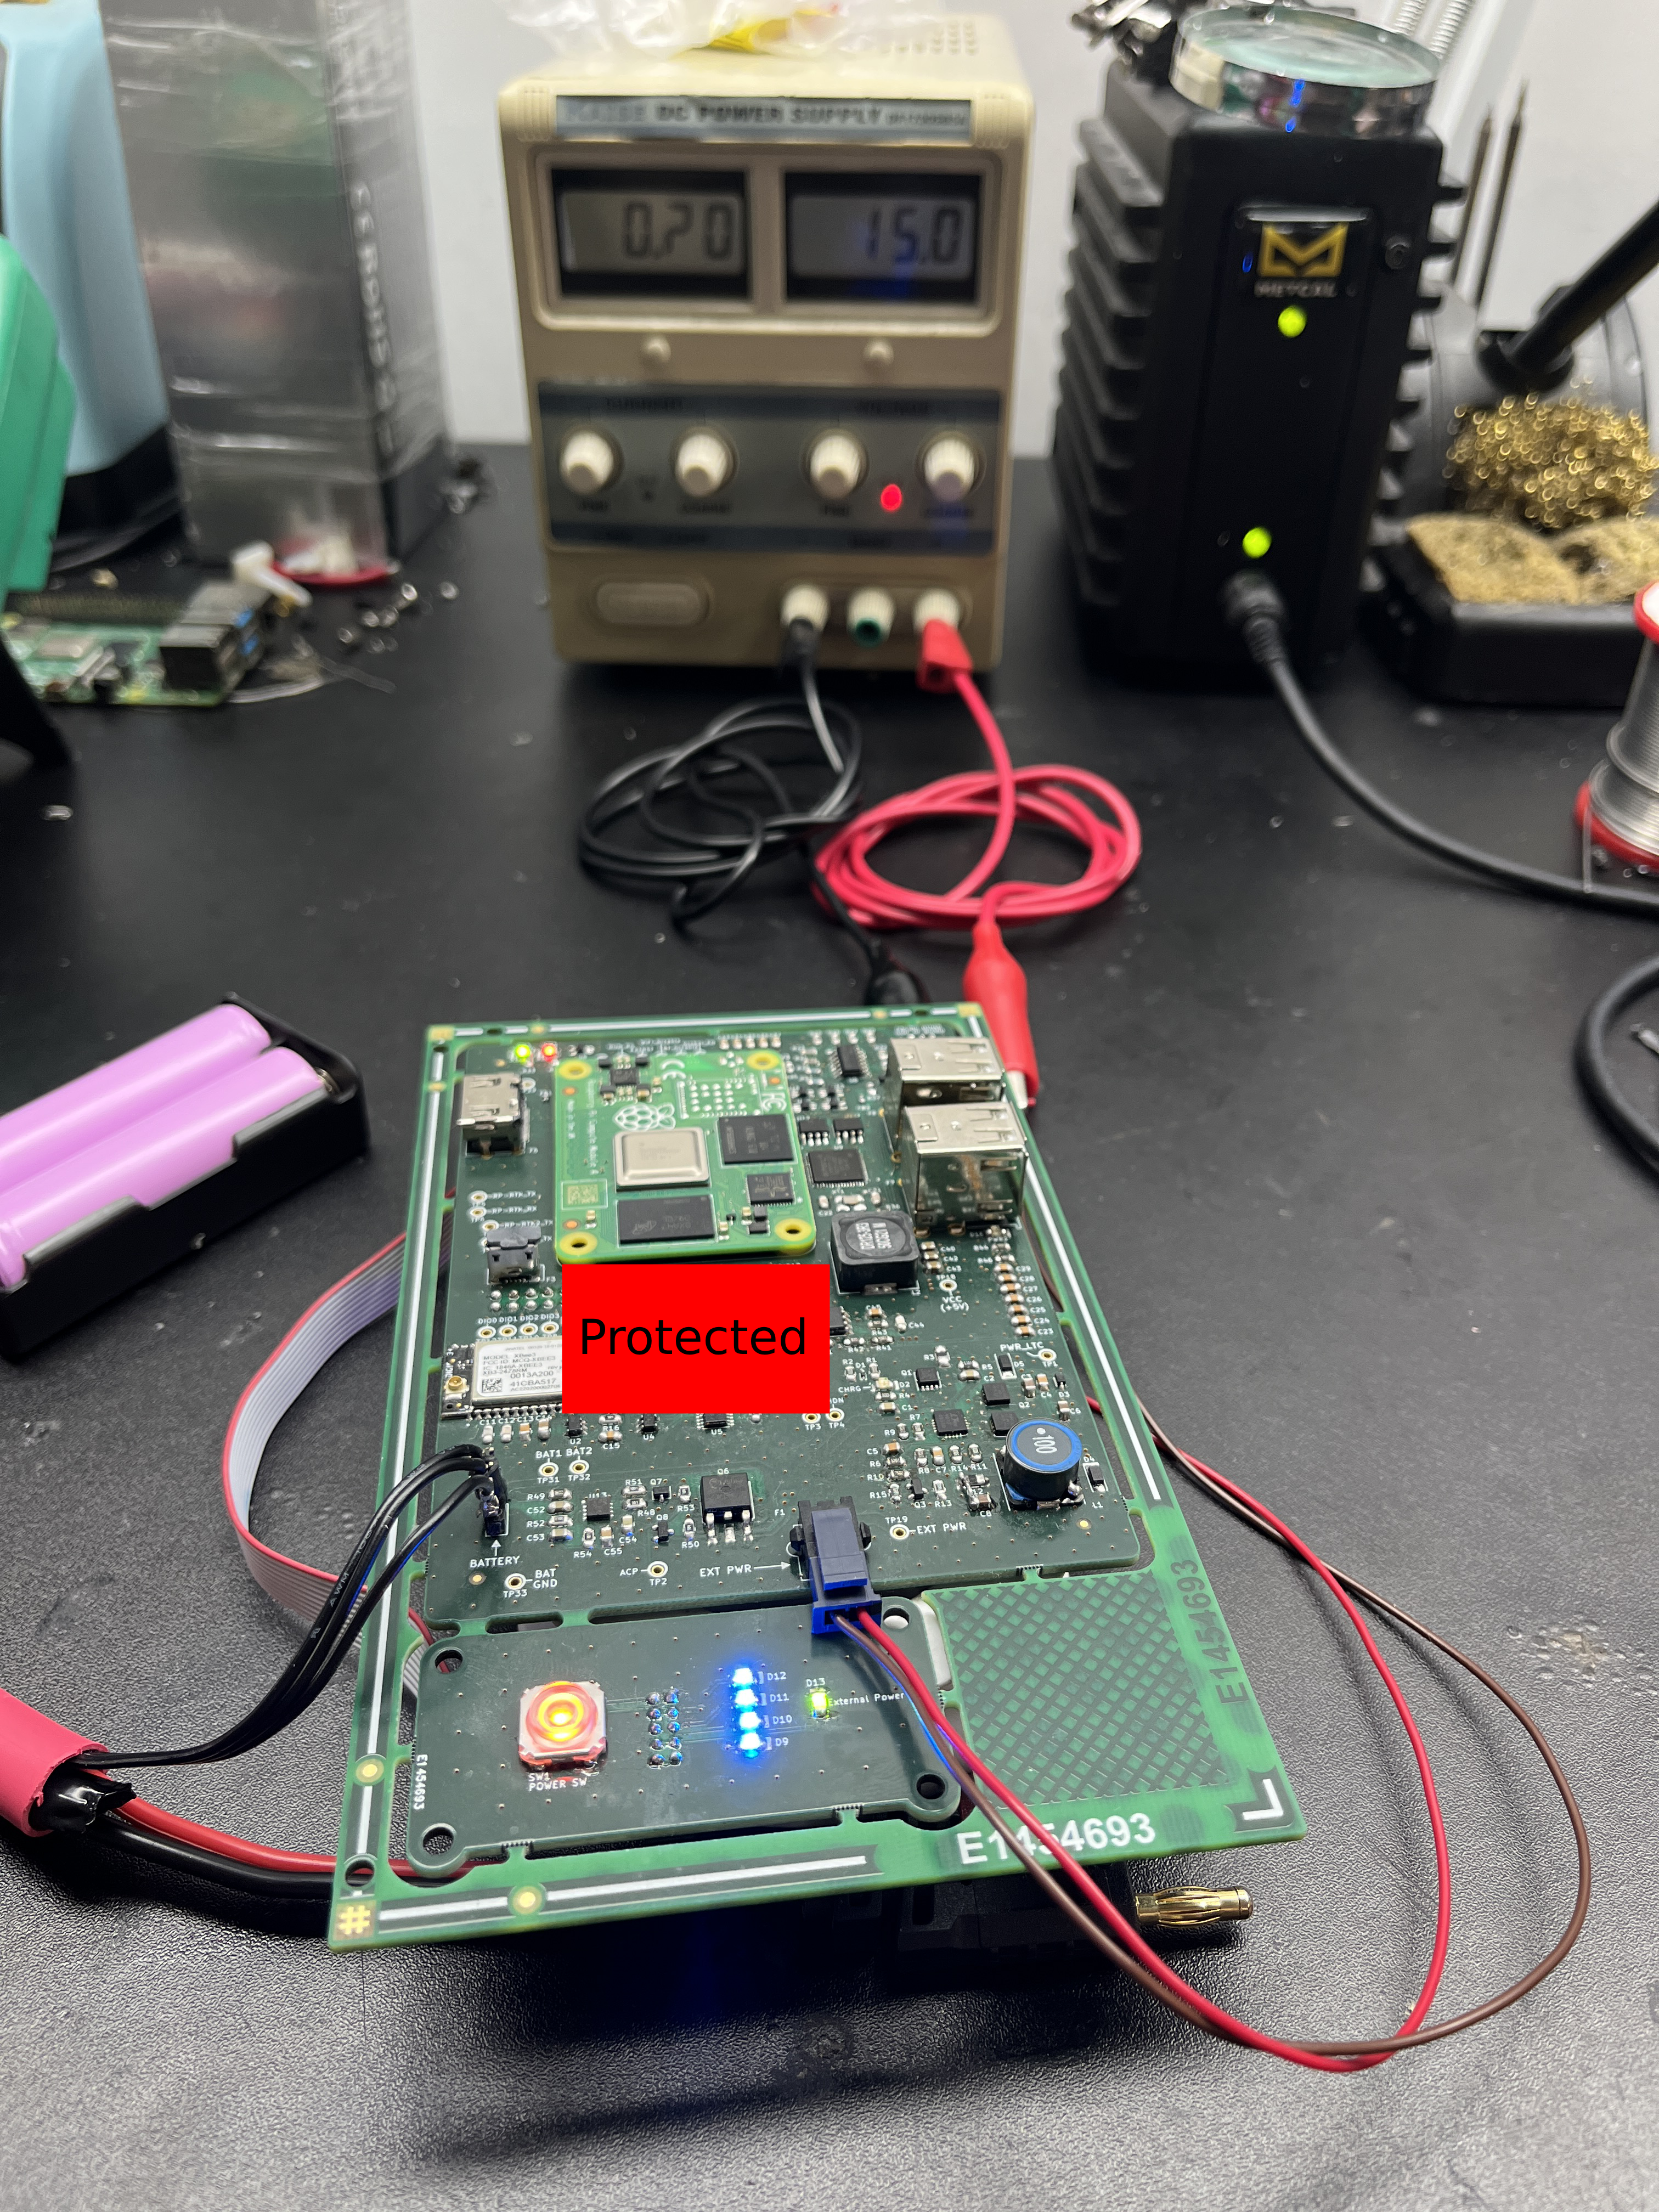
\includegraphics[width=0.7\textwidth]{Chapters/Figures/chapter5/prototype/7_consumo.png}
	\caption{Functional testing of the new beRTK\textsuperscript{\textregistered} PCB (external power and battery pack power applied; with the Raspberry Pi CM4).}
	\label{fig:7_consumo}
\end{figure}% 7_consumo

%depois é que falo dos LEDs de Activity e PWR
Also visible on all operation modes are the lighting events of both activity and power LEDs for the CM4, as soon as the power switch is pressed (Figure~\ref{fig:7_consumo}). Before using the CM4, only the power LED lit up (Figure~\ref{fig:5_proto_first_test_ONLY_EXT_PWR}) -- which was the expected behaviour since this LED's power is controlled by an inverter fed with the 5V from the AP64501 output net, as seen in Figure~\ref{fig:CM4_GPIO_circuit}.

\begingroup
\begin{table}[h]
	\caption{CM4 GPIO circuit's most relevant voltages expected and measured, for all operational modes, with the CM4 mounted on the prototype.}
	\label{tab:CM4_GPIO_3_modes_WITH_CM4}
	\centering
	\resizebox{\textwidth}{!}{%
	\begin{tabular}{lcccccc}
        \toprule
		\multicolumn{7}{c}{\textbf{CM4 GPIO Circuit (CM4 mounted on the board)}} \\
		\midrule
        {} & \multicolumn{2}{c}{\textbf{Mode 1}} & \multicolumn{2}{c}{\textbf{Mode 2}} & \multicolumn{2}{c}{\textbf{Mode 3}} \\
		\midrule
		{} & \textbf{Exp. (V)} & \textbf{Meas. (V)} & \textbf{Exp. (V)} & \textbf{Meas. (V)} & \textbf{Exp. (V)} & \textbf{Meas. (V)} \\
		\midrule
		\textbf{+5V} 			& $5.00$  & $5.01$  & $5.00$  & $5.01$  & $5.00$  & $5.01$ \\
        \midrule
		\textbf{+3V3} 			& $3.30$ & $3.30$ & $3.30$ & $3.30$ & $3.30$ & $3.30$ \\
        \midrule
		\textbf{Global\_EN} 	& $5.00$ & $4.82$ & $5.00$ & $4.82$ & $5.00$ & $4.82$ \\
        \midrule
		\textbf{RUN\_PG} 		& $3.30$ & $3.29$ & $3.30$ & $3.28$ & $3.30$ & $3.29$ \\
		\midrule
		\textbf{nEXTRST} 		& $3.30$ & $3.29$ & $3.30$ & $3.28$ & $3.30$ & $3.29$ \\
		\midrule
		% \textbf{WL\_nDisable} 	& $0.00$ & $0.00$ & $0.00$ & $0.00$ & $0.00$ & $0.00$ \\
		% \midrule
		% \textbf{BT\_nDisable} 	& $0.00$ & $0.00$ & $0.00$ & $0.00$ & $0.00$ & $0.00$ \\
		% \midrule
		\textbf{GPIO12} 		& $0.00$ & $0.03$ & $0.00$ & $0.02$ & $0.00$ & $0.03$ \\
		\midrule
		\textbf{GPIO13}			& $0.00$ & $0.02$ & $0.00$ & $0.02$ & $0.00$ & $0.02$ \\
		\midrule
		\textbf{GPIO18}			& $0.00$ & $0.01$ & $0.00$ & $0.01$ & $0.00$ & $0.01$ \\
		\midrule
		\textbf{GPIO19}			& $0.00$ & $0.01$ & $0.00$ & $0.01$ & $0.00$ & $0.01$ \\
		\midrule
		\textbf{GPIO20}			& $0.00$ & $0.03$ & $0.00$ & $0.03$ & $0.00$ & $0.03$ \\
		\midrule
		\textbf{GPIO21}			& $0.00$ & $0.01$ & $0.00$ & $0.01$ & $0.00$ & $0.01$ \\
        \bottomrule
    \end{tabular}}
\end{table}
\endgroup% CM4_GPIO_3_modes_WITH_CM4

\begingroup
\begin{table}[h]
	\caption{CM4 high-speed circuit's most relevant voltages expected and measured, for all operational modes, with the CM4 mounted on the prototype.}
	\label{tab:CM4_HighSpeed_3_modes_WITH_CM4}
	\centering
	\resizebox{\textwidth}{!}{%
	\begin{tabular}{lcccccc}
        \toprule
		\multicolumn{7}{c}{\textbf{CM4 High-Speed Circuit (CM4 mounted on the board)}} \\
		\midrule
        {} & \multicolumn{2}{c}{\textbf{Mode 1}} & \multicolumn{2}{c}{\textbf{Mode 2}} & \multicolumn{2}{c}{\textbf{Mode 3}} \\
		\midrule
		{} & \textbf{Exp. (V)} & \textbf{Meas. (V)} & \textbf{Exp. (V)} & \textbf{Meas. (V)} & \textbf{Exp. (V)} & \textbf{Meas. (V)} \\
		\midrule
		\textbf{USB\_OTG\_ID} 	& $0.00$ & $0.00$ & $0.00$ & $0.00$ & $0.00$ & $0.00$ \\
        \midrule
		\textbf{HDMI\_5V} 		& $5.00$ & $5.01$ & $5.00$ & $5.01$ & $5.00$ & $5.01$ \\
        \bottomrule
    \end{tabular}}
\end{table}
\endgroup% CM4_HighSpeed_3_modes_WITH_CM4

The expected values were obtained while measuring the relevant voltages for both connector sides of the CM4, and an established 3.3V net was verified. The HDMI side of the board was also correctly powered.

Before accurate readings on the LAN9514 hub can be done, the CM4 must first be set up. If this is not done, the device will not provide it's intended capabilities, among which is the USB interface. Figure~\ref{fig:HDMI_CM4_not_working} shows the first attempt at connecting the prototype to an external monitor through an HDMI cable. It was successful, since the connection was clearly established without any HDMI-related problems; the monitor screen displays a typical message of a CM4 without an operating system installed: ``SD: card not detected''.

\begin{figure}[h]
	\centering
	\includegraphics[width=0.7\textwidth]{Chapters/Figures/chapter5/prototype/HDMI_CM4_not_working.png}
	\caption{First HDMI test of the new beRTK\textsuperscript{\textregistered} PCB (CM4 without the Raspberry Pi OS installed).}
	\label{fig:HDMI_CM4_not_working}
\end{figure}% HDMI_CM4_not_working

The CM4 version used on the prototype provides an eMMC flash module installed, and therefore an external SD card was not needed -- the Raspberry Pi OS can simply be installed directly on the module itself. For that, as explained in Section~\ref{sec:3234_LAN9514}, either an upstream USB port or the CM4IO development board can be used -- the latter option was taken, since an upstream USB port was not implemented on the prototype and the CM4IO was available during the development stage of the project. Figure~\ref{fig:9_proto_CM4IO} shows the CM4 mounted on the CM4IO board, connected to a PC via a Micro-USB cable in order to install the Raspberry Pi OS on the module.

\begin{figure}[h]
	\centering
	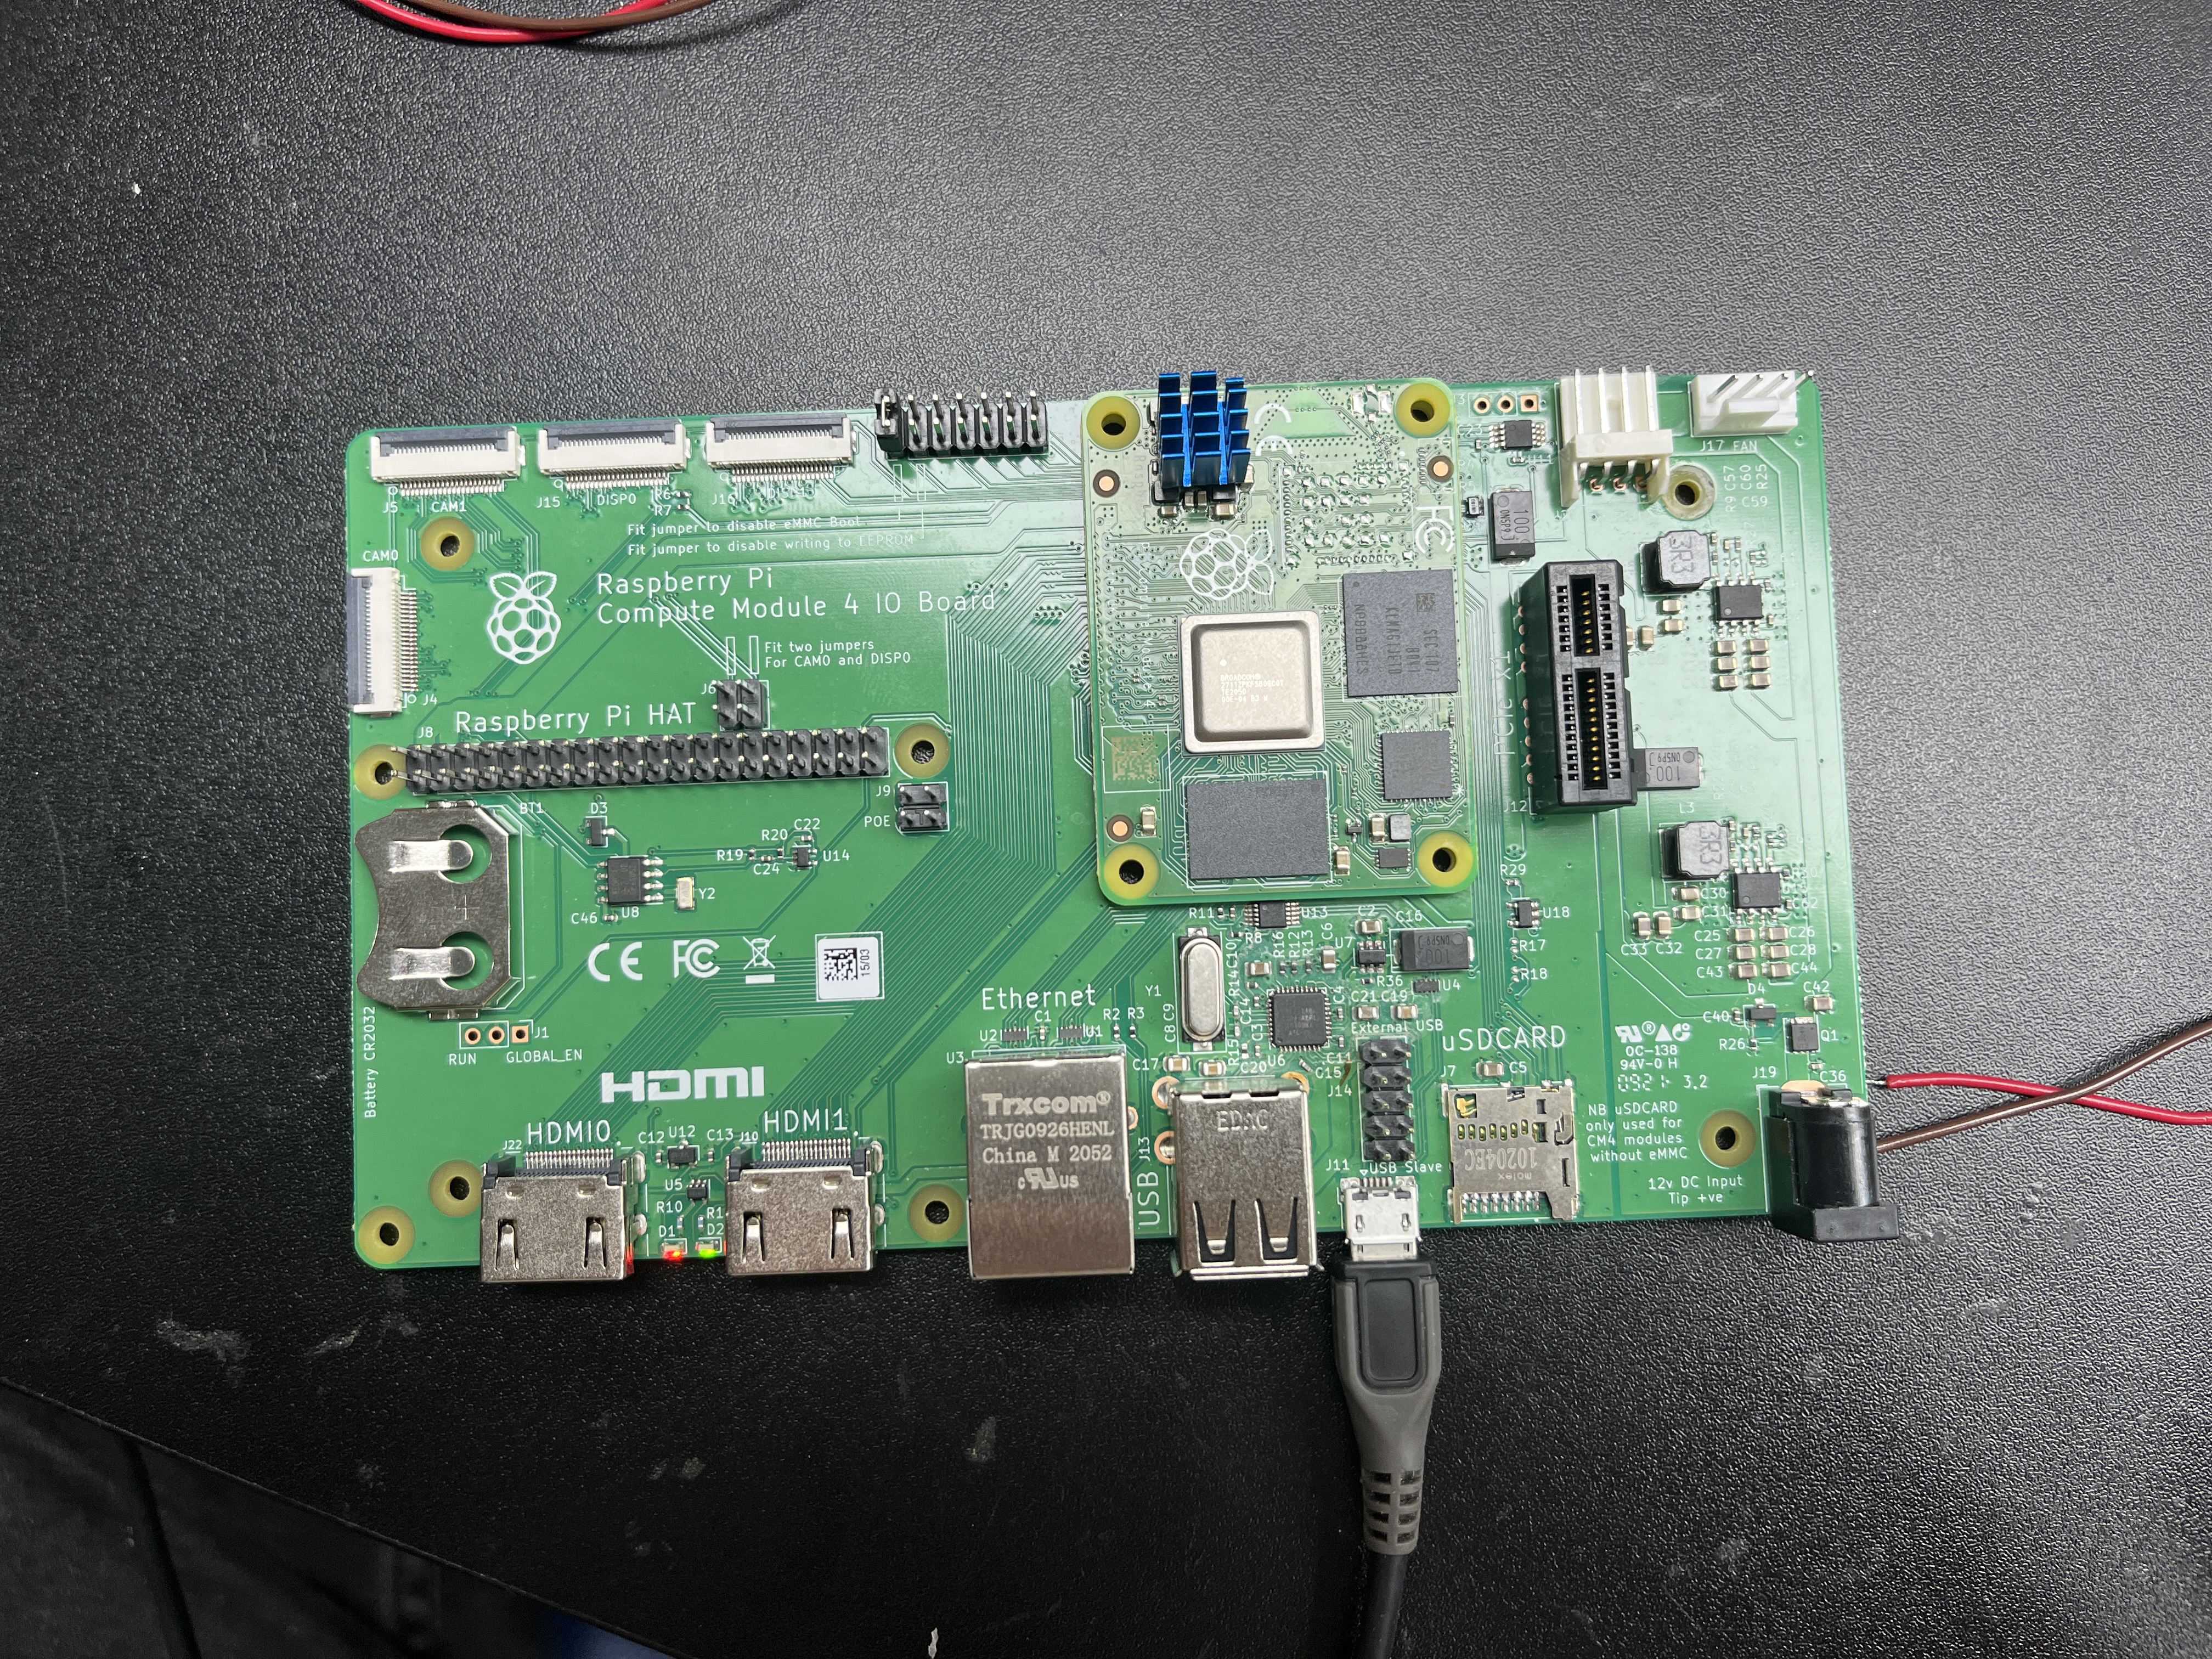
\includegraphics[width=0.7\textwidth]{Chapters/Figures/chapter5/prototype/9_proto_CM4IO.png}
	\caption{Installing the Raspberry Pi OS on the CM4, using the CM4IO board.}
	\label{fig:9_proto_CM4IO}
\end{figure}% 9_proto_CM4IO

Connecting the prototype once again to an external monitor using an HDMI cable reveals the operating system was correctly installed on the module, which is now operational, as shown in Figure~\ref{fig:10_proto_HDMI_and_RPiOS_working}.

\begin{figure}[h]
	\centering
	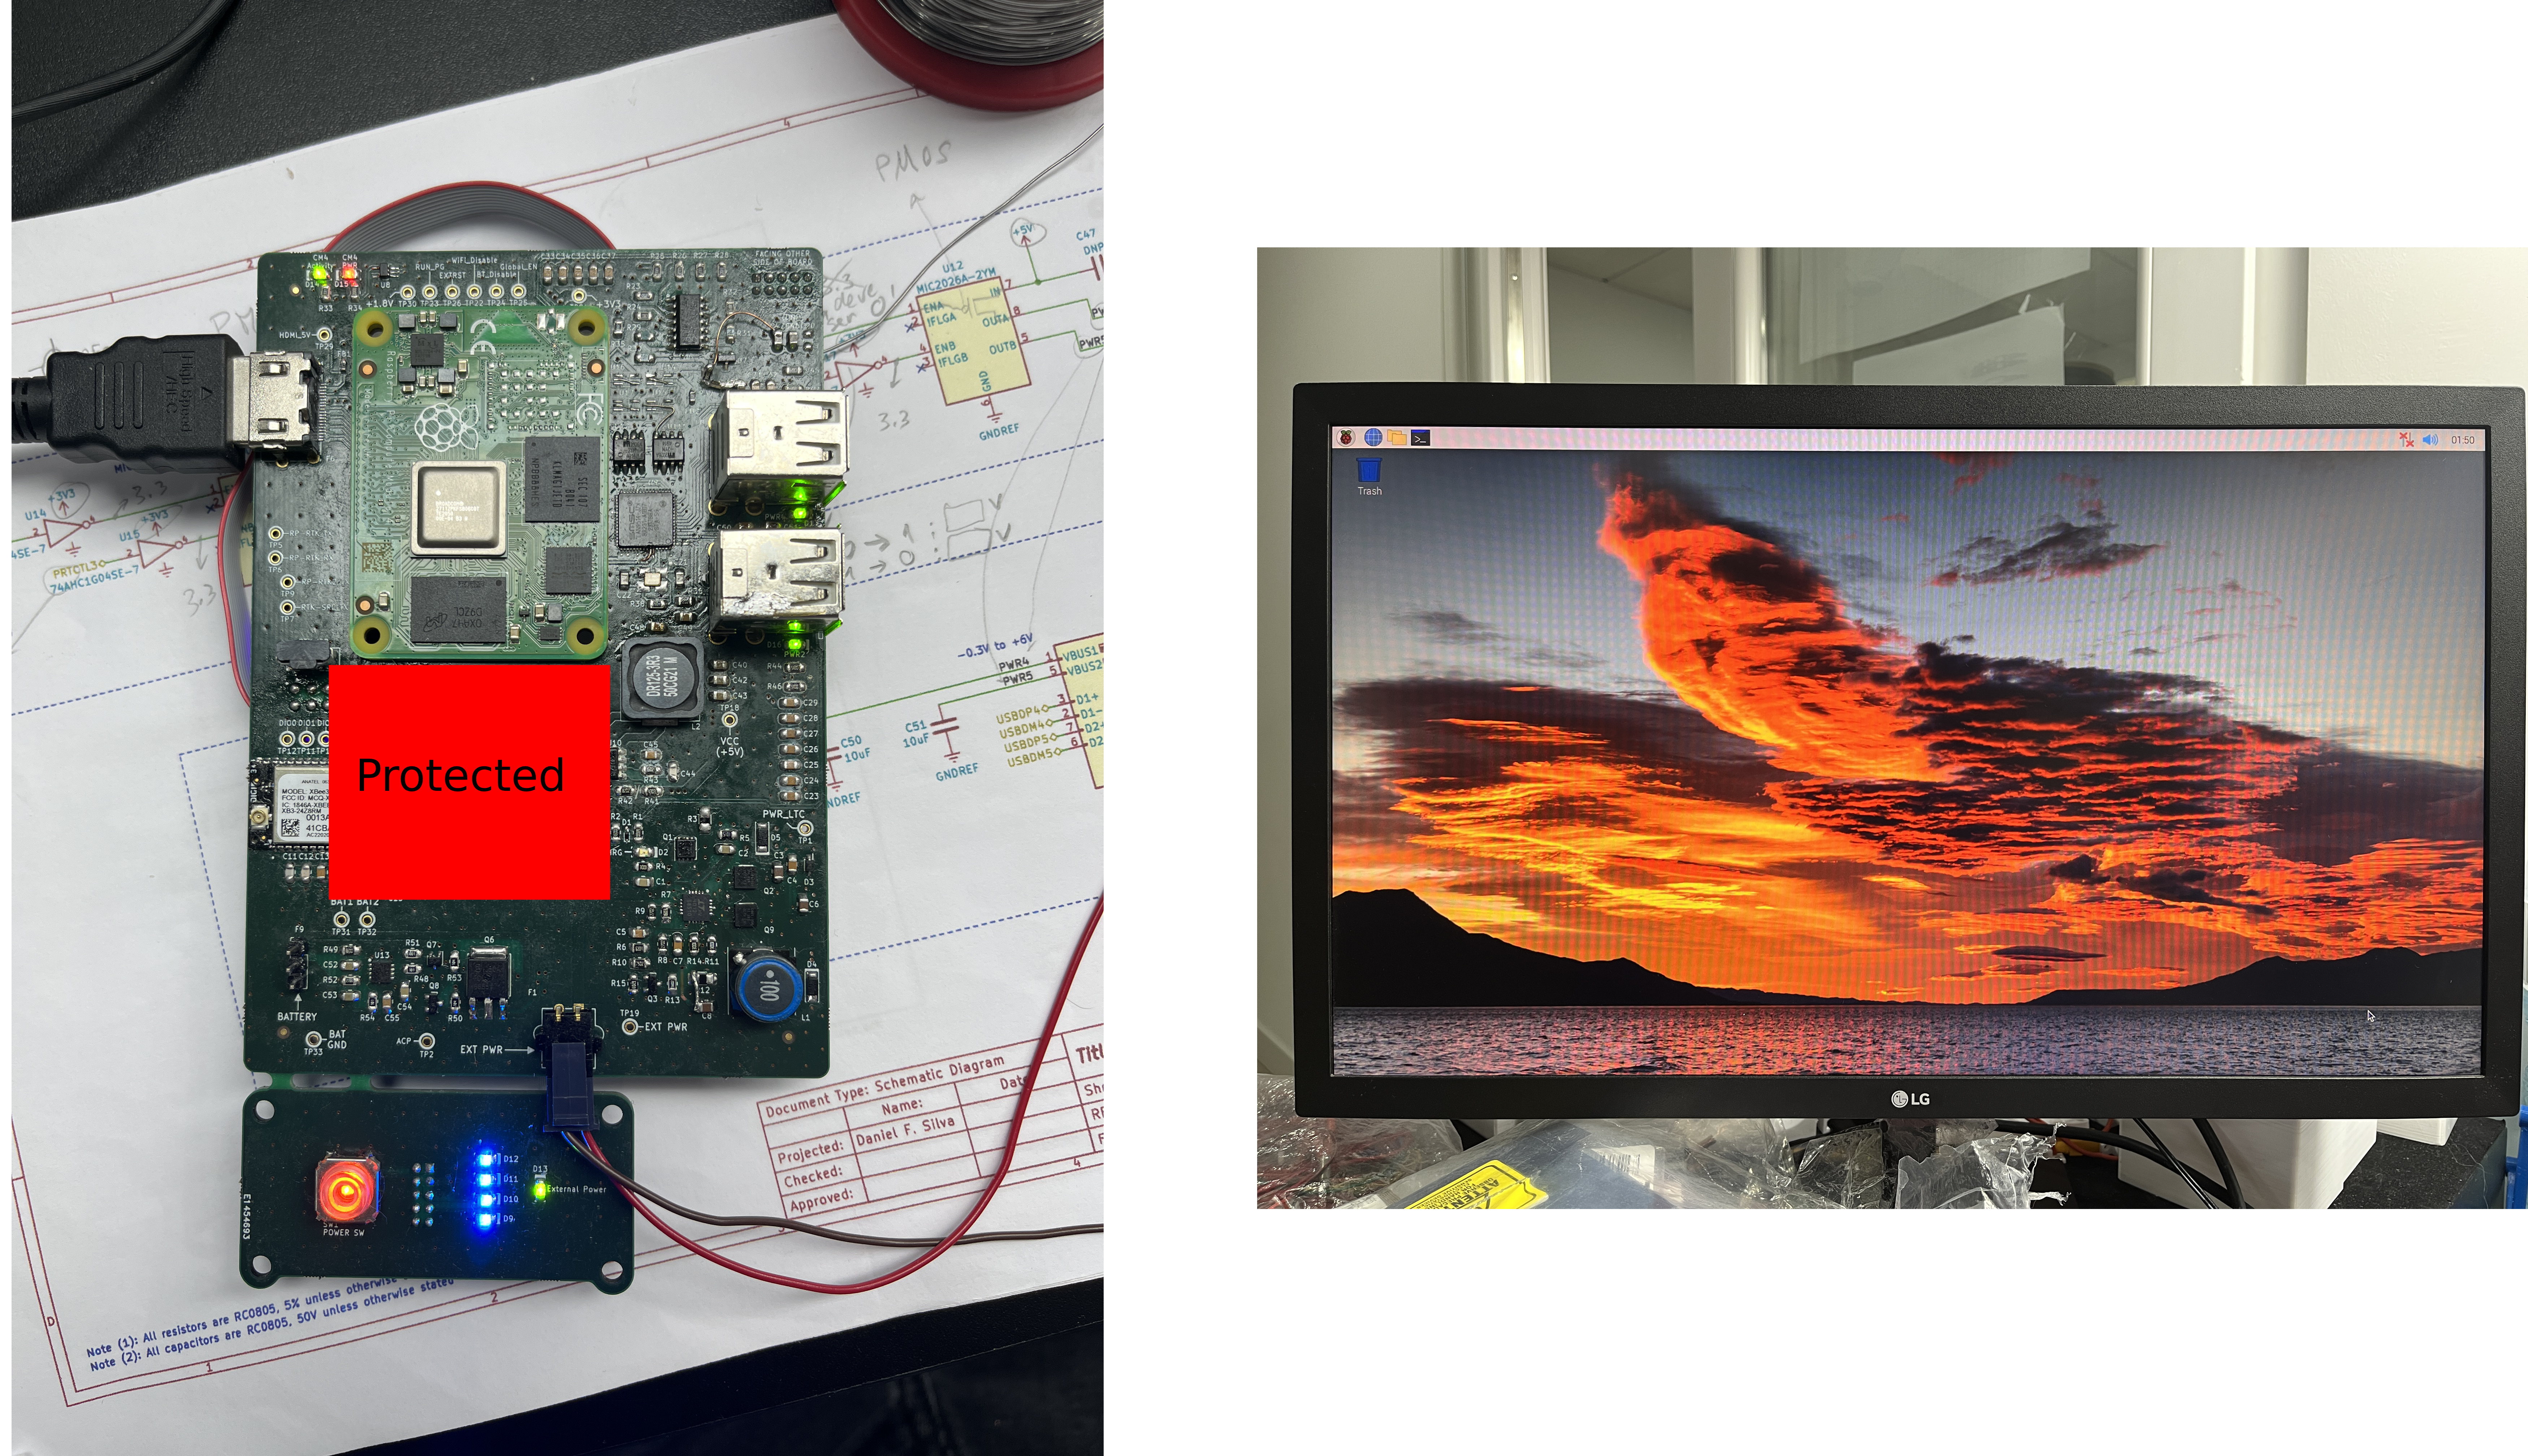
\includegraphics[width=0.7\textwidth]{Chapters/Figures/chapter5/prototype/10_proto_HDMI_and_RPiOS_working.png}
	\caption{HDMI test of the new beRTK\textsuperscript{\textregistered} PCB (CM4 with the Raspberry Pi OS installed).}
	\label{fig:10_proto_HDMI_and_RPiOS_working}
\end{figure}% 10_proto_HDMI_and_RPiOS_working

Table~\ref{tab:LAN9514_3_modes_WITH_CM4} highlights, for all three operational modes, the most relevant voltages expected and measured for the LAN9514 hub, with a CM4 loaded with the Raspberry Pi OS mounted on the board.

% agora podem-se tirar as medidas do LAN9514:
\begingroup
\begin{table}[h]
	\caption{LAN9514 and downstream ports circuits' most relevant voltages expected and measured, for all operational modes, with the CM4 mounted on the prototype.}
	\label{tab:LAN9514_3_modes_WITH_CM4}
	\centering
	\resizebox{\textwidth}{!}{%
	\begin{tabular}{lcccccc}
        \toprule
		\multicolumn{7}{c}{\textbf{LAN9514 Circuit (CM4 mounted on the board)}} \\
		\midrule
        {} & \multicolumn{2}{c}{\textbf{Mode 1}} & \multicolumn{2}{c}{\textbf{Mode 2}} & \multicolumn{2}{c}{\textbf{Mode 3}} \\
		\midrule
		{} & \textbf{Exp. (V)} & \textbf{Meas. (V)} & \textbf{Exp. (V)} & \textbf{Meas. (V)} & \textbf{Exp. (V)} & \textbf{Meas. (V)} \\
		\midrule
		\textbf{VDD33IO} 	& $3.30$ & $3.30$ & $3.30$ & $3.30$ & $3.30$ & $3.30$ \\
        \midrule
		\textbf{VDD33A} 	& $3.30$ & $3.29$ & $3.30$ & $3.29$ & $3.30$ & $3.29$ \\
        \midrule
		\textbf{VDD18CORE} 	& $1.80$ & $1.80$ & $1.80$ & $1.80$ & $1.80$ & $1.80$ \\
		\midrule
		\textbf{IN -- U11} 	& $5.00$ & $5.01$ & $5.00$ & $5.01$ & $5.00$ & $5.01$ \\
		\midrule % port 1
		\textbf{PRTCTL2} 	& $3.30$ & $0.85$ & $3.30$ & $0.85$ & $3.30$ & $0.85$ \\
		\midrule
		\textbf{ENA -- U11} & $0.00$ & $3.29$ & $0.00$ & $3.31$ & $0.00$ & $3.29$ \\
		\midrule
		\textbf{PWR2} 		& $5.00$ & $0.02$ & $5.00$ & $0.01$ & $5.00$ & $0.02$ \\
		\midrule % port 2
		\textbf{PRTCTL3} 	& $3.30$ & $0.82$ & $3.30$ & $0.82$ & $3.30$ & $0.82$ \\
		\midrule
		\textbf{ENB -- U11} & $0.00$ & $3.28$ & $0.00$ & $3.30$ & $0.00$ & $3.28$ \\
		\midrule
		\textbf{PWR3} 		& $5.00$ & $0.01$ & $5.00$ & $0.01$ & $5.00$ & $0.01$ \\
		\midrule		
		\textbf{IN -- U12} 	& $5.00$ & $5.01$ & $5.00$ & $5.01$ & $5.00$ & $5.01$ \\
		\midrule % port 3
		\textbf{PRTCTL4} 	& $3.30$ & $0.79$ & $3.30$ & $0.79$ & $3.30$ & $0.79$ \\
		\midrule
		\textbf{ENA -- U12} & $0.00$ & $3.31$ & $0.00$ & $3.31$ & $0.00$ & $3.31$ \\
		\midrule
		\textbf{PWR4} 		& $5.00$ & $0.02$ & $5.00$ & $0.02$ & $5.00$ & $0.01$ \\
		\midrule % port 4
		\textbf{PRTCTL5} 	& $3.30$ & $0.81$ & $3.30$ & $0.81$ & $3.30$ & $0.81$ \\
		\midrule
		\textbf{ENB -- U12} & $0.00$ & $3.29$ & $0.00$ & $3.28$ & $0.00$ & $3.29$ \\
		\midrule
		\textbf{PWR5} 		& $5.00$ & $0.01$ & $5.00$ & $0.01$ & $5.00$ & $0.01$ \\
        \bottomrule
    \end{tabular}}
\end{table}
\endgroup% LAN9514_3_modes_WITH_CM4

Analysing the values on Table~\ref{tab:LAN9514_3_modes_WITH_CM4}, it can be noticed that, even though the voltages on all power pins seem to be correct, the voltages on the four USB port power control pins (PRTCTLx) are not.

Before any conclusion could be drawn, the correct functioning of the 25MHz crystal oscillator needed to be verified. For that, using a digital oscilloscope, the crystal's oscillation frequency was measured, as shown in Figure~\ref{fig:25MHz_oscilloscope}.

\begin{figure}[h]
	\centering
	\includegraphics[width=0.7\textwidth]{Chapters/Figures/chapter5/prototype/25MHz_oscilloscope.png}
	\caption{LAN9514 25MHz crystal oscillator frequency measurement using a digital oscilloscope.}
	\label{fig:25MHz_oscilloscope}
\end{figure}% 25MHz_oscilloscope

As seen in Figure~\ref{fig:25MHz_oscilloscope}, it is possible to read and verify the waveform for the expected 25MHz from the crystal oscillator. The waveform observed also seems to have little to no amount of disturbances.

All power pins were also monitored afterwards to check for the presence of noise, and even though a small amount of disturbances were found, these were concluded as not critical for the correct functioning of the hub. 

Since the LAN9514 relies on the CM4 in order to communicate via USB, the CM4 datahseet (\cite{CM4}) informs the user that the module's USB interface is disabled by default on the firmware, in order to save power. However, in recent versions of the Raspberry Pi OS, it is automatically enabled by a single code line -- \verb!otg_mode=1! -- in a configurations file named ``config.txt''. Mounting the CM4 back on the CM4IO board and checking the config.txt file, the line ``\verb!otg_mode=1!'' was indeed verified to be in the file.

As for the remaining LAN9514's USB-related pins -- VBUS\_DET, USBRBIAS, VDD18USBPLL and every data signal pin --, these were verified (with respect to the schematic and layout design) together with the IC's datasheet~\cite{LAN9514}, hardware design checklist manual~\cite{LAN9514_HW_Design_Checklist}, and reference schematic~\cite{LAN9514_ref_schematic}, in order to comply with the specific design requirements for the project. With this, while observing the home screen to the CM4's operating system, connecting a mouse and keyboard to the downstream USB ports of the prototype reported no feedback. Noting once more~\cite{CM4} and~\cite{LAN9514}, it can be concluded that the issue may be related to the lack of a more precise way to set the CM4 as a host or device. Without this definition the USB data transit through the downstream ports appears impossible.

Referring back to the circuit schematic of the USB downstream ports (Figure~\ref{fig:USB_Hub_Downstream_circuit}) exposed in Section~\ref{sec:3234_LAN9514}, it can be seen that each PRTCTL pin connects to the input of a 74AHC1G04 single inverter gate. Subsequently, each inverter controls a single enable pin of a MIC2026A-2YM USB port power controller, which controls the flow of power to each USB downstream port. As previously mentioned, this inverter is placed before the enable pin to counter its active-low nature -- as the MIC2026-1BM USB port power controller, which has an active-high enable pin, suggested by~\cite{LAN9514_ref_schematic}, was not available at the prototyping stage of the project. Analysing Section 5.2.3 of the LAN9514 hardware design checklist manual (\cite{LAN9514_HW_Design_Checklist}), a graphical representation for a typical downstream VBUS port power control implementation can be found. Figure~\ref{fig:VBUS_HW_Design_Chklst} displays such representation.

\begin{figure}[h]
	\centering
	\includegraphics[width=0.7\textwidth]{Chapters/Figures/chapter5/prototype/VBUS_HW_Design_Chklst.pdf}
	\caption{Typical downstream VBUS port power control implementation~\cite{LAN9514_HW_Design_Checklist}.}
	\label{fig:VBUS_HW_Design_Chklst}
\end{figure}% VBUS_HW_Design_Chklst

\cite{LAN9514_HW_Design_Checklist} also informs the user that the typical implementation shown in Figure~\ref{fig:VBUS_HW_Design_Chklst} assumes a port power controller with an active-high enable input and an active-low, open-drain style fault indicator (for the sensing of overcurrent conditions). It also mentions that ``external polarity inversion through buffers or FETs may be required if the port power controller has different I/O characteristics.'', which is the reason for the implementation of a 74AHC1G04 single inverter gate on both enable inputs of the selected MIC2026A-2YM port power controllers.

However, there is a conflict of information when reviewing another document made available by the manufacturer of the LAN9514: the schematic checklist. In the schematic guidelines' section for the USB downstream interface port 2, the document states that ``\dots care must be taken when selecting a power distribution switch for the LAN9514. Power distribution switches are available with active-high enables or active-low enables. Active-low enable parts will not work with our combined Fault/Enable PRTCTL2 pin. The power distribution switch must have an active-high enable input and an overcurrent fault indication active-low output.''~\cite{LAN9514_Schematic_Checklist}; the same statements are made for each of the remaining three USB downstream interface ports. Figure~\ref{fig:VBUS_Schematic_Chklst} displays a representation of a typical LAN9514 USB downstream port application found in~\cite{LAN9514_Schematic_Checklist}. Comparing such representation to the one previously shown in Figure~\ref{fig:VBUS_HW_Design_Chklst}, the similarities are clear. Granted the schematic checklist document -- last revised in 2013 --, is older than the hardware design checklist document -- which in turn was last revised in 2022 --, the information seems to clash and may inevitably be prone to some design questions.

\begin{figure}[h]
	\centering
	\includegraphics[width=0.7\textwidth]{Chapters/Figures/chapter5/prototype/VBUS_Schematic_Chklst.pdf}
	\caption{Typical LAN9514 USB downstream port application~\cite{LAN9514_Schematic_Checklist}.}
	\label{fig:VBUS_Schematic_Chklst}
\end{figure}% VBUS_Schematic_Chklst

From what can ultimately be described as a design flaw, the testing of the prototype had to be stopped at the USB data transfer stage. Since this interface is critical to the performance of the new beRTK\textsuperscript{\textregistered} base station, it cannot be bypassed in any way. Redesign of the LAN9514 and CM4 high-speed circuits are necessary in order to solve the issues described and be able to advance to the project's next step.




%modos de operação:
%1: só EXT power -- tensao no terminal BAT do LTC4012 passa como se fosse CLN (ou a tensao exterior), e como ACP vs 5V ainda é suficiente para ligar o PMOS switch Q8,Q6, a status voltage passa na mesma e assim acendem os LEDs na mesma. - solução: fazer o R14,D6,Q4
%2: EXT power + baterias
%3: só baterias - diminuir a luz de um LED no photoshop para mostrar que os LEDs iam apagando



% -- As mentioned before, the top and bottom power FETs Q2 and Q9, along with inductor L1 are vital to the PWM control architecture. These components are part of the sub-circuit that starts from the +15VDC source of power and passes across FET Q1 (connected to pin INFET), sense resistor R3, 
% This sub-circuit forms the ``power supply rail'', and upon layout design of the circuit from Figure~\ref{fig:LTC4012_circuit}, this section must bear a track width large enough to withstand large values of currents or any other phenomena that may occur (e.g. voltage/current spikes). The needed track width can be calculated through the following expression:

% XBee: Digi XBee 3 RF Module Hardware Reference Manual
% We design XBee 3 RF Modules to be self-sufficient and have minimal sensitivity to nearby processors,
% crystals or other printed circuit board (PCB) components. Keep power and ground traces thicker than
% signal traces and make sure that they are able to comfortably support the maximum current
% specifications. There are no other special PCB design considerations to integrate XBee 3 RF Modules,
% with the exception of antennas.




%LTC4012:
% It should be noted that, for the top and bottom FET selection stage, the Si7212DN model suggested is a double FET in one package. The CSD17308Q3 substituting model is a single-channel FET (only one per package), and therefore two units had to be acquired -- Section~\ref{sec:3211_LTC4012}.




    % inductor L2:
    % Meter Eq. 9 do datasheet do AP64501;
    
    % Peak current determines the required saturation current rating, which influences the size of the inductor. Saturating the inductor decreases the converter efficiency while increasing the temperatures of the inductor and the internal power MOSFETs. Therefore, choosing an inductor with the appropriate saturation current rating is important. 
    % It is recommended by \cite{AP64501} the selection of an inductor value between $1 \mu$H to $10 \mu$H, and therefore, taking into account the values presented in Table~\ref{tab:AP64501_recommended_values}, an inductor of $3.6 \mu$H was selected. It is also advised to select an indcutor with a DC current rating of at least 35\% higher than the maximum 5A load current of the AP64501, which corresponds to 6.75A.
    % For highest efficiency, the inductor's DC resistance should be less than 10mOhm. Use a larger inductance for improved efficiency under light load conditions.






%-------------------------------
% Basicamente o processo de fazer uma base rtk de zero é simples:
% 	- O software é instalares o OS e depois fazeres clone da tal git.
% 	- Na git estão as instruções de como instalar o software todo. É só seguir e está feito.
% 	- É possível que tenhas de trocar uma porta nos parâmetros ou algo assim porque em vez do wi-fi estar na USB3 está na USB1 ou algo assim, mas não há de ser muito mais que isso.
% 	- Ya podes fazer uma imagem clean no teu rpi e instalar tudo como se fosse uma base rtk.
% Depois no fim fazes uma imagem clean again só para não ficares com a tralha.